% =========================================================================
% A Mathematical Model of Channels, Carriers, and Runtime Vocabulary Genesis
% Tech-report style, single column, IEEEtran
% =========================================================================
\documentclass[journal,onecolumn,11pt]{IEEEtran}

% --- packages -------------------------------------------------------------
\usepackage[margin=1in]{geometry}
\usepackage{amsmath,amssymb,amsthm}
\usepackage{microtype}
\usepackage{hyperref}
\usepackage{cleveref}
\usepackage{tikz}
\usetikzlibrary{positioning,arrows.meta,shapes.geometric,calc,fit,backgrounds}
\usepackage{booktabs}
\usepackage{tabularx}
\usepackage{longtable}
\usepackage{ragged2e}
\usepackage{enumitem}
\usepackage{xcolor}

% --- table column types ---------------------------------------------------
\newcolumntype{L}[1]{>{\RaggedRight\arraybackslash}p{#1}}
\newcolumntype{Y}{>{\RaggedRight\arraybackslash}X}

% --- theorem environments (sequential numbering, IEEE style) --------------
\theoremstyle{definition}
\newtheorem{definition}{Definition}
\newtheorem{lemma}{Lemma}
\newtheorem{theorem}{Theorem}

% --- hyperref styling -----------------------------------------------------
\hypersetup{
  colorlinks=true,
  linkcolor=blue!55!black,
  citecolor=blue!55!black,
  urlcolor=blue!55!black,
  pdftitle={A Mathematical Model of Channels, Carriers, and Runtime Vocabulary Genesis},
  pdfauthor={Liam McGuire}
}

% --- TikZ block style -----------------------------------------------------
\tikzset{
  block/.style={
    draw, rounded corners, fill=blue!6,
    minimum height=9mm, minimum width=22mm,
    align=center, font=\small, inner sep=1.5mm
  },
  branchblock/.style={
    draw, rounded corners, fill=orange!10,
    minimum height=9mm, minimum width=24mm,
    align=center, font=\small, inner sep=1.5mm
  },
  endblock/.style={
    draw, rounded corners, fill=green!8,
    minimum height=9mm, minimum width=24mm,
    align=center, font=\small, inner sep=1.5mm
  },
  arrow/.style={-{Latex[length=2mm,width=2mm]}, thick}
}

% --- notation-table helper -----------------------------------------------
% A consistent mini-table format for per-section notation tables.
\newcommand{\notationtable}[3]{%
  \begin{table}[ht]
  \centering
  \caption{#1}
  \label{#2}
  \small
  \renewcommand{\arraystretch}{1.1}
  \begin{tabularx}{\linewidth}{L{0.22\linewidth} L{0.27\linewidth} Y}
  \toprule
  Symbol & Inhabits / Type & Meaning \\
  \midrule
  #3
  \bottomrule
  \end{tabularx}
  \end{table}%
}

% --- title block ----------------------------------------------------------
\title{A Mathematical Model of Channels, Carriers,\\and Runtime Vocabulary Genesis}
\author{Liam McGuire\\
\textit{Independent Researcher}\\
\href{mailto:liammcg44@gmail.com}{liammcg44@gmail.com}\\
\textbf{Technical Report} \\
April 2026}

\begin{document}
\maketitle

\begin{abstract}
We define a substrate-agnostic mathematical model of quantitative simulations whose vocabulary may be extended at runtime through recorded events. State is organised into \emph{channels}---real-valued scalars hosted by \emph{carriers}---that combine within a tick under a small operator algebra and drift between ticks under a per-carrier-permitted family of dynamical regimes. The model's distinctive feature is a transition that admits new channels into the registry between ticks under a quality--diversity admission rule, with a lineage log whose closure ensures every entry traces in finitely many recorded steps to a fixed seed set. We extend this with a \emph{revision} transition that permits the redefinition of existing channels through branching lineage, while preserving the closure property. Properties (determinism, registry monolithicism, emergence closure) are stated as constructive consequences of the model's signatures; design choices are discussed in a concluding rationale.
\end{abstract}

\begin{IEEEkeywords}
open-ended evolution, simulation modelling, runtime vocabulary, lineage closure, quality--diversity, Indian buffet process, agent-based simulation, evolutionary computation
\end{IEEEkeywords}

% =========================================================================
\section{Background}
\label{sec:background}

Modern simulation systems --- games, scientific models, agent-based artificial life --- increasingly aim at \emph{open-ended} dynamics: behaviour that is not fully prescribed at design time but emerges from the runtime interaction of many small components. This places a particular demand on the simulation's representational substrate: it must be expressive enough to admit phenomena the designer did not anticipate, while remaining structured enough to permit determinism, replay, and verification. The model we present is an attempt to satisfy both demands within a single mathematical framework.

Three lines of prior work converge on the present model.

The first is the gene-regulatory-network tradition in evolutionary computation, originating with quantitative-genetics models and elaborated by Wagner~\cite{wagner2011} for evolutionary innovation and by Stanley~\cite{stanley2007} for compositional pattern-producing networks. Here, \emph{channels} --- real-valued scalars under bounded ranges --- combine according to learnable circuits to produce phenotypes. The model in this paper inherits the channels-as-bounded-scalars premise and the separation of \emph{what is a signal} from \emph{how signals combine}.

The second is the gameplay-attribute systems used in commercial game engines, where a small operator vocabulary (additive, multiplicative, threshold, gating, antagonistic) is sufficient to express most observed mechanics. We adopt this operator set unchanged. The economic and materials-fatigue literatures supply the analogous between-tick dynamics --- monotonic wear, mean-reverting decay, first-order momentum, scheduled forcing --- which we generalise under a single drift signature.

The third, and the most relevant to the paper's distinctive contribution, is the open-ended-evolution literature. Soros and Stanley~\cite{soros2014} identify four necessary conditions for open-endedness; the Indian Buffet Process of Griffiths and Ghahramani~\cite{griffiths2011} provides the canonical mathematical object for unbounded latent-feature discovery; the Bayesian Program Learning of Lake et al.~\cite{lake2015} formalises compositional concept formation; the quality--diversity admission rules of Lehman and Stanley~\cite{lehman2011} and Mouret and Clune~\cite{mouret2015}, refined more recently by Lim et al.~\cite{lim2025}, provide bounded archives of diverse candidates; the activity-score classification of Bedau, Snyder, and Packard~\cite{bedau1998} provides an evolutionary garbage-collection criterion; the constructivist schema-mechanism tradition initiated by Drescher~\cite{drescher1991} (after Piaget) supplies the spin-off statistics that drive when a new feature should be hypothesised. Our genesis transition is constructed to simultaneously satisfy Soros and Stanley's conditions while drawing on each of these contributions.

The contribution of the present paper is to unify these strands into a single substrate-agnostic mathematical model whose registry-extension semantics admit a closure theorem (\cref{thm:lineage}) and whose extension to redefinition (\cref{thm:lineage-rev}) preserves that closure. We have in mind the simulation of biological--cultural co-evolution at multiple scales --- genome, behaviour, language, technology, ideology --- within a single deterministic framework, but the model itself is independent of that domain.

% =========================================================================
\section{Preliminaries}
\label{sec:notation}

We work in discrete time with tick counter $t \in \mathbb{N}$. Each subsequent section introduces the symbols local to it in a small notation table at the start of the section. \Cref{tab:notation-prelim} collects only the universally-used symbols.

A bar over a quantity ($\bar{q}$) denotes a registered \emph{kind} (a type-like object); the corresponding plain symbol is an \emph{instance} of that kind. Two minor overloadings are flagged in their per-section tables: $r$ doubles as the running value in a composition operator and as a revision-event tuple, and $\Delta$ doubles as a drift list ($\Delta_C$) and as a semantic-distance witness ($\Delta_r$). Both are always disambiguated by context.

\notationtable{Universal symbols.}{tab:notation-prelim}{
$\mathbb{R}$              & ---                          & real values; channel and parameter values live here \\
$\mathbb{N}$              & ---                          & natural numbers; tick indices live here \\
$\mathbb{I}$              & ---                          & a countable set of identifier strings \\
$\mathbb{B} = \{0,1\}$    & ---                          & predicate values \\
$t$                       & $\mathbb{N}$                 & the current tick \\
$[\![\varphi]\!]$         & $\mathbb{B}$                 & Iverson bracket: $1$ if $\varphi$ holds, else $0$ \\
$\mathrm{clamp}_{[a,b]}(x)$ & $\mathbb{R}$               & projection $\max(a, \min(b, x))$ \\
$\bigwedge$               & operator                     & boolean conjunction (empty conjunction $=1$) \\
$\bigsqcup$               & operator                     & disjoint union of sets \\
$\biguplus$               & operator                     & multi-set disjoint union \\
$\bar{q}$                 & convention                   & a registered \emph{kind} (e.g., $\bar{g}$, $\bar{d}$); plain $q$ is an instance \\
}

% =========================================================================
\section{Channels and Carriers}
\label{sec:channels}

The model has two atomic objects, defined below. \Cref{tab:notation-channels} collects the symbols introduced here.

\notationtable{Symbols introduced in \cref{sec:channels}.}{tab:notation-channels}{
$B$                       & $\mathcal{B}$                & a carrier \\
$\mathcal{B}$             & finite set                   & the carrier registry, frozen at simulation start \\
$\mathrm{id}_B$           & $\mathbb{I}$                 & carrier identifier \\
$\bar{D}_B$               & $\subseteq \mathrm{dom}(\bar{\mathcal{D}})$ & drift kinds permitted on $B$ \\
$\bar{G}_B$               & $\subseteq \mathrm{dom}(\bar{\mathcal{G}})$ & gate kinds permitted on $B$ \\
$S_B$                     & $\subset \mathbb{I}$, finite & substrate-site enumeration of $B$ \\
$\lambda_B$               & specification                & birth/death/inheritance hooks for instances of $B$ \\
$C$                       & $\mathcal{C}_t$              & a channel \\
$\mathcal{C}_t$           & set                          & channel registry at tick $t$ (extensible by genesis) \\
$\mathrm{id}_C$           & $\mathbb{I}$                 & channel identifier (unique within carrier) \\
$B_C$                     & $\mathcal{B}$                & carrier of $C$ \\
$R_C$                     & $\subset \mathbb{R}$         & range $[\underline{r}_C, \overline{r}_C]$ \\
$\underline{r}_C, \overline{r}_C$ & $\mathbb{R}$         & lower and upper range bounds of $C$ \\
$\Delta_C$                & ordered list                 & drift-instance list of $C$ \\
$H_C$                     & ordered list                 & composition-hook list of $C$ \\
$\Gamma_C$                & finite set                   & gate-instance set of $C$ \\
$\pi_C$                   & $\Pi$                        & provenance string of $C$ \\
$\Pi$                     & regular language             & provenance grammar (extended later in \cref{sec:revision}) \\
}

A carrier is the ``kind of thing that hosts state.'' A genome is one carrier; a settlement is another; a piece of equipment is a third. Each kind of host comes with a fixed personality: which kinds of randomness make sense for its values (mutation for genomes, wear for artefacts, institutional drift for collectives), which world conditions it can be sensitive to (biomes, mount slots, fiscal year), and which spatial sites its values can be attached to (limbs, ward, sword parts). The carrier is the \emph{type-level} declaration; particular genomes, settlements, and items are \emph{instances} of it.

\begin{definition}[Carrier]\label{def:carrier}
A \emph{carrier} is a tuple
\[
B \;=\; \langle\, \mathrm{id}_B,\; \bar{D}_B,\; \bar{G}_B,\; S_B,\; \lambda_B \,\rangle
\]
where $\mathrm{id}_B \in \mathbb{I}$; $\bar{D}_B \subseteq \mathrm{dom}(\bar{\mathcal{D}})$ and $\bar{G}_B \subseteq \mathrm{dom}(\bar{\mathcal{G}})$ are finite sets of permitted drift-operator and gate kinds; $S_B \subset \mathbb{I}$ is a finite (possibly empty) set of substrate sites; and $\lambda_B$ specifies how instances of $B$ are born and destroyed. The carrier registry $\mathcal{B}$ is a finite set of carriers, fixed for the life of the simulation.
\end{definition}

A channel is the simplest possible piece of dynamic state in the model: one real number with a minimum and maximum. The other fields tell the kernel, separately, how it changes between ticks (drift), how it combines with other channels within a tick (hooks), when it applies (gates), and where it came from (provenance). The channel itself doesn't \emph{do} any of those things; it just stores the number. The kernel reads the other fields when scheduling work.

\begin{definition}[Channel]\label{def:channel}
A \emph{channel} is a tuple
\[
C \;=\; \langle\, \mathrm{id}_C,\; B_C,\; R_C,\; \Delta_C,\; H_C,\; \Gamma_C,\; \pi_C \,\rangle
\]
where $B_C \in \mathcal{B}$; $R_C = [\underline{r}_C, \overline{r}_C] \subset \mathbb{R}$; $\Delta_C$ is an ordered list of drift instances each with $k_\delta \in \bar{D}_{B_C}$; $H_C$ is an ordered list of composition hooks; $\Gamma_C$ is a set of gate instances each with $k_\gamma \in \bar{G}_{B_C}$; and $\pi_C \in \Pi$ is the provenance.
\end{definition}

Channel ids are unique within a carrier but not globally: the channel registry $\mathcal{C}$ is keyed by the pair $(\mathrm{id}_{B_C}, \mathrm{id}_C)$.

The asymmetry between the two objects is intentional. Carriers fix what \emph{kinds of dynamics} are permitted; channels are the dumb scalars on which those dynamics actually run. A channel knows nothing about how it changes (the role of its drift instances) or about when it applies (the role of its gates).

% =========================================================================
\section{The State Space}
\label{sec:state}

\notationtable{Symbols introduced in \cref{sec:state}.}{tab:notation-state}{
$i$                       & $I_t(B)$                     & a live instance of carrier $B$ at tick $t$ \\
$I_t(B)$                  & finite set                   & live instances of $B$ at tick $t$ \\
$s$                       & $S_B \cup \{\bot\}$          & a substrate site of $B$, or ``no site'' \\
$\bot$                    & ---                          & the ``no site'' marker \\
$S_C$                     & $\subseteq S_{B_C}$          & site subset declared by $C$'s substrate-site gate, if any \\
$x_C^{(i,s,t)}$           & $R_C$ or $R_C^{S_C}$         & raw value of $C$ on instance $i$ at site $s$, tick $t$ \\
$\sigma_t(B,i)$           & finite map                   & instance state: channel id $\mapsto$ raw value or site map \\
$\Sigma_t$                & $\bigsqcup_{B,i}\sigma_t(B,i)$ & world channel state at tick $t$ \\
$E_t$                     & opaque                       & environment at tick $t$ (read-only) \\
}

Most channels are just one number per instance. A few are spatially distributed across substrate sites --- a creature may have different sensitivity per body part; a sword has different durability per component --- and those carry a small site-indexed map instead of a scalar. Whether a particular channel takes the scalar form or the per-site form is decided by whether its gate set includes a substrate-site gate.

\begin{definition}[Raw channel value]\label{def:raw}
Let $S_C \subseteq S_{B_C}$ be the (possibly empty) site set declared by the substrate-site gate of $C$, if any. The raw value of $C$ on instance $i$ at tick $t$ is
\[
x_C^{(i,\cdot,t)} \;\in\;
\begin{cases}
R_C & \text{if } S_C = \emptyset,\\
R_C^{S_C} & \text{otherwise (a finite site-indexed map).}
\end{cases}
\]
\end{definition}

The state of a single carrier instance --- one particular genome, settlement, or sword --- collects the raw values of every channel that lives on the carrier of that instance. The world's state is then the disjoint union over all instances of all carriers; this is the object that gets serialised when the simulation saves.

\begin{definition}[Instance state]
The state of instance $i$ of carrier $B$ at tick $t$ is the finite map
\[
\sigma_t(B,i) \;:\; \{C \in \mathcal{C}_t \mid B_C = B\} \;\longrightarrow\; \text{(scalar or site-indexed map)}
\]
respecting \cref{def:raw}.
\end{definition}

\begin{definition}[World channel state]
\[
\Sigma_t \;=\; \bigsqcup_{B \in \mathcal{B}}\;\bigsqcup_{i \in I_t(B)}\; \sigma_t(B,i).
\]
\end{definition}

We assume an environment $E_t$ --- a read-only structure recording auxiliary state needed by gates and drift; its internal type is opaque to the model.

% =========================================================================
\section{Gates and Effective Values}
\label{sec:gates}

A gate makes a channel either \emph{active} (its raw value flows downstream) or \emph{dormant} (it contributes zero). Gates are pure predicates --- no randomness, no side effects.

\notationtable{Symbols introduced in \cref{sec:gates}.}{tab:notation-gates}{
$\bar{g}$                 & $\mathrm{dom}(\bar{\mathcal{G}})$ & a gate kind \\
$\Theta_{\bar{g}}$        & a type                       & parameter type for kind $\bar{g}$ \\
$\phi_{\bar{g}}$          & predicate                    & predicate function of kind $\bar{g}$ \\
$\gamma$                  & $\Gamma_C$                   & a gate instance \\
$k_\gamma$                & $\bar{G}_{B_C}$              & gate kind referenced by $\gamma$ \\
$\theta_\gamma$           & $\Theta_{k_\gamma}$          & parameter value of $\gamma$ \\
$\Phi_C(\sigma, E, s)$    & $\mathbb{B}$                 & activeness predicate of $C$ \\
$\hat{x}_C^{(i,s,t)}$     & $R_C$                        & effective value of $C$ at $(i,s,t)$ \\
}

A gate kind is a registered ``question we can ask about the world.'' The biome gate kind asks ``is this entity in a forest?''; the body-part kind asks ``is this channel applying at the head?''; the seasonal kind asks ``is it winter?'' Each kind comes with its own parameter type --- the biome kind takes a flag string, the body-part kind takes a list of site ids --- and a pure predicate over carrier state, environment, and (optionally) the current site.

\begin{definition}[Gate kind]
A gate kind $\bar{g}$ is a triple $\langle \mathrm{id}_{\bar{g}}, \Theta_{\bar{g}}, \phi_{\bar{g}}\rangle$ where $\Theta_{\bar{g}}$ is a parameter type and
\[
\phi_{\bar{g}} \;:\; \Theta_{\bar{g}} \times \mathrm{State} \times \mathrm{Env} \times (S \cup \{\bot\}) \;\to\; \mathbb{B}.
\]
A gate instance $\gamma$ on channel $C$ supplies a kind $k_\gamma \in \bar{G}_{B_C}$ and a parameter value $\theta_\gamma \in \Theta_{k_\gamma}$.
\end{definition}

A channel is \emph{active} iff every gate attached to it answers ``yes.'' This is just a Boolean conjunction: any single gate failing makes the channel dormant for that instance and site.

\begin{definition}[Channel activeness]
\[
\Phi_C\bigl(\sigma_t(B_C,i),\, E_t,\, s\bigr) \;:=\; \bigwedge_{\gamma \in \Gamma_C}\, \phi_{k_\gamma}\!\bigl(\theta_\gamma,\, \sigma_t(B_C,i),\, E_t,\, s\bigr).
\]
The empty conjunction is $1$, so a channel with no gates is always active.
\end{definition}

When a channel is active, its effective value is its raw value clamped to the legal range; when it is dormant, the effective value is zero. Sending dormant channels to zero (rather than removing them entirely) is a small choice with a big payoff: every operator downstream becomes total, with no special cases for ``the channel didn't apply.''

\begin{definition}[Effective value]\label{def:effective}
Write $\sigma$ for $\sigma_t(B_C,i)$. The effective value of $C$ at site $s$ is
\[
\hat{x}_C^{(i,s,t)} \;:=\; \Phi_C(\sigma,E_t,s) \cdot \mathrm{clamp}_{R_C}\!\bigl(x_C^{(i,s,t)}\bigr).
\]
A dormant channel contributes effective value $0$; the raw value is unchanged and persists in $\sigma$.
\end{definition}

% =========================================================================
\section{Composition}
\label{sec:compose}

Within a tick, channels combine. The composition law is a deterministic left fold over a totally-ordered list of binary operators.

\notationtable{Symbols introduced in \cref{sec:compose}.}{tab:notation-compose}{
$h$                       & $H_C$                        & a composition hook \\
$\mathrm{id}_h$           & $\mathbb{I}$                 & hook identifier (used to sort the fold) \\
$\kappa_h$                & $\{\mathrm{add},\mathrm{mul},\mathrm{thr},\mathrm{gate},\mathrm{ant}\}$ & hook kind \\
$\mathrm{partner}(h)$     & $\mathcal{C}_t$              & partner channel referenced by $h$ \\
$k_h$                     & $\mathbb{R}$                 & coefficient of $h$ \\
$\tau_h$                  & $\mathbb{R}$                 & threshold of $h$ \\
$\mathrm{emits}(h)$       & $\subseteq \mathcal{P}_t$    & primitives emitted by $h$ \\
$\eta_\kappa$             & $\mathbb{R}^4 \to \mathbb{R}$ & operator semantics for kind $\kappa$ \\
$r$                       & $\mathbb{R}$                 & running value parameter in $\eta_\kappa$ (overloaded with revision event $r$, \cref{sec:revision}) \\
$c$                       & $\mathbb{R}$                 & partner's effective value parameter in $\eta_\kappa$ \\
$k$                       & $\mathbb{R}$                 & coefficient parameter in $\eta_\kappa$ \\
$\tau$                    & $\mathbb{R}$                 & threshold parameter in $\eta_\kappa$ \\
$r_j$                     & $R_C$                        & running value at fold step $j$ \\
$\mathcal{E}_C$           & $R_C$                        & composed effective value of $C$ at site $s$ \\
}

A composition hook is a single ingredient in the recipe for combining channels: ``given your current value, pull from your partner channel, scaled by this coefficient, gated by this threshold, in this style (additive, multiplicative, threshold, gate, antagonistic).'' Channels stack hooks the way the gameplay-attribute systems of commercial engines stack modifiers --- a fact we exploit deliberately, since that vocabulary turns out to be enough.

\begin{definition}[Composition hook]
A composition hook is
\[
h \;=\; \langle\, \mathrm{id}_h,\; \kappa_h,\; \mathrm{partner}(h),\; k_h,\; \tau_h,\; \mathrm{emits}(h) \,\rangle
\]
where $\kappa_h \in \{\mathrm{add},\mathrm{mul},\mathrm{thr},\mathrm{gate},\mathrm{ant}\}$; $\mathrm{partner}(h) \in \mathcal{C}_t$ identifies a partner channel on the same carrier; $k_h \in \mathbb{R}$ is a coefficient; $\tau_h \in \mathbb{R}$ is a threshold; and $\mathrm{emits}(h) \subseteq \mathcal{P}_t$ is a (possibly empty) emission set.
\end{definition}

The five operator kinds are simple. \emph{Additive} and \emph{multiplicative} are the workhorses: stacking contributions and scaling. \emph{Threshold} introduces conditional behaviour --- the partner has to clear a bar before contributing. \emph{Gating} is a binary on/off switch driven by the partner. \emph{Antagonistic} is subtraction. We claim no novelty in this vocabulary; it is essentially the gameplay-attribute kit, kept because empirically it covers what most simulations need.

\begin{definition}[Operator semantics]\label{def:opsem}
Each kind $\kappa$ defines a binary operator $\eta_\kappa$ taking a running value $r$, a partner value $c$, a coefficient $k$, and a threshold $\tau$:
\begin{align*}
\eta_{\mathrm{add}}(r,c;k,\tau) &= r + kc, &
\eta_{\mathrm{mul}}(r,c;k,\tau) &= r\,(1+kc), \\
\eta_{\mathrm{thr}}(r,c;k,\tau) &= r + [\![c \ge \tau]\!]\, kc, &
\eta_{\mathrm{gate}}(r,c;k,\tau) &= [\![c \ge \tau]\!]\, r, \\
\eta_{\mathrm{ant}}(r,c;k,\tau) &= r - kc.
\end{align*}
\end{definition}

The hooks combine in sequence, sorted by their identifier. The fold starts at the channel's effective value, applies each hook one at a time, and clamps to the channel's range after each step. There is nothing special about sort-by-id as an order; we just need \emph{some} fixed deterministic order, and id-sort is the cheapest one that reproduces across runs and machines.

\begin{definition}[Composition fold]
Sort $H_C$ by $\mathrm{id}_h$ ascending: $H_C = (h_1 < h_2 < \cdots < h_n)$. Define the recurrence
\[
r_0 = \hat{x}_C^{(i,s,t)}, \qquad
r_j = \mathrm{clamp}_{R_C}\!\Bigl(\eta_{\kappa_{h_j}}\!\bigl(r_{j-1},\, \hat{x}_{\mathrm{partner}(h_j)}^{(i,s,t)};\; k_{h_j},\, \tau_{h_j}\bigr)\Bigr).
\]
The \emph{composed effective value} is $\mathcal{E}_C(\sigma,E,s) := r_n$.
\end{definition}

Because each step is a deterministic function of the previous value and the partner's effective value, and the order of steps is fixed by hook id, there is no freedom for runtime scheduling to perturb the answer. This is what we make precise next.

\begin{lemma}[Determinism of composition]\label{lem:comp-det}
$\mathcal{E}_C$ is a deterministic function of $(\sigma, E, s)$ and the registries.
\end{lemma}

\begin{proof}
$H_C$ is sorted by hook id; $\hat{x}$ depends only on $(\sigma, E, s)$ by \cref{def:effective}; each $\eta_\kappa$ is a total real-valued function. Composition of total deterministic functions is total and deterministic.
\end{proof}

A cyclic dependency --- channels whose hooks reference each other through \texttt{partner-of} --- is rejected at validation time, except for an opt-in fixed-point fold with a declared iteration cap and tolerance.

% =========================================================================
\section{Drift}
\label{sec:drift}

Between ticks, raw values change. The change is governed by drift operators, which generalise mutation, wear, decay, momentum, and scheduled forcing under a single signature.

\notationtable{Symbols introduced in \cref{sec:drift}.}{tab:notation-drift}{
$\bar{d}$                 & $\mathrm{dom}(\bar{\mathcal{D}})$ & a drift-operator kind \\
$\Theta_{\bar{d}}$        & a type                       & parameter type for kind $\bar{d}$ \\
$f_{\bar{d}}$             & function                     & drift update function of kind $\bar{d}$ \\
$\beta_{\bar{d}}$         & $\{\mathrm{clamp},\mathrm{reflect},\mathrm{wrap}\}$ & bounds policy of kind $\bar{d}$ \\
$\delta$                  & $\Delta_C$                   & a drift instance \\
$k_\delta$                & $\bar{D}_{B_C}$              & drift kind referenced by $\delta$ \\
$\theta_\delta$           & $\Theta_{k_\delta}$          & parameter value of $\delta$ \\
$\Omega$                  & abstract space               & PRNG-state space; one stream per subsystem \\
$\omega^t$                & $\Omega$                     & PRNG state at tick $t$ \\
$\mathcal{D}_C$           & function                     & drift fold operator of $C$ \\
$y_j, y'_j$               & $\mathbb{R}$                 & intermediate raw values inside $\mathcal{D}_C$ \\
$\omega_j$                & $\Omega$                     & intermediate PRNG state inside $\mathcal{D}_C$ \\
}

Where gates ask Boolean questions, drift kinds describe \emph{change-over-time recipes}: Gaussian noise, monotonic wear, mean-reverting decay, momentum, scheduled forcing. Each kind takes a real-valued state, advances it by one tick, and threads pseudorandom state through. Crucially, this is the only place stochasticity enters the model --- everything else is deterministic given inputs.

\begin{definition}[Drift kind]
A drift kind $\bar{d}$ is
\[
\bar{d} \;=\; \langle\, \mathrm{id}_{\bar{d}},\; \Theta_{\bar{d}},\; f_{\bar{d}},\; \beta_{\bar{d}} \,\rangle
\]
where $\Theta_{\bar{d}}$ is a parameter type, $\beta_{\bar{d}} \in \{\mathrm{clamp},\mathrm{reflect},\mathrm{wrap}\}$ is a bounds policy, and
\[
f_{\bar{d}} \;:\; \mathbb{R} \times \Theta_{\bar{d}} \times \mathrm{State} \times \mathrm{Env} \times \Omega \;\to\; \mathbb{R} \times \Omega.
\]
$\Omega$ is an abstract state of pseudorandom information; $f_{\bar{d}}$ may consume and advance it. We require the model to be \emph{stream-deterministic}: the function $f_{\bar{d}}$ depends only on its inputs, and the $\Omega$ it threads is a per-subsystem stream seeded once at simulation start. (This is the only place randomness enters the model.)
\end{definition}

After drift, the new value might land outside the legal range. The bounds policy is the recipe for handling that: clamp to the boundary, reflect off it, or wrap modulo the range width. Clamp is the default and matches most physical readings of what ``out-of-range'' should mean.

\begin{definition}[Bounds policy]
\[
\beta_{\mathrm{clamp},R}(x) = \mathrm{clamp}_R(x),\quad
\beta_{\mathrm{wrap},[a,b]}(x) = a + ((x-a) \bmod (b-a)),
\]
with $\beta_{\mathrm{reflect}}$ defined by piecewise reflection at the endpoints (omitted).
\end{definition}

A channel may stack multiple drift instances --- e.g., Gaussian mutation \emph{plus} a scheduled seasonal forcing. They apply one after another, like a pipeline: each takes the previous value, advances it, applies its bounds policy. The result is the channel's raw value at tick $t+1$.

\begin{definition}[Drift step]\label{def:drift}
For channel $C$ on instance $i$, with $\Delta_C = (\delta_1, \ldots, \delta_m)$ in declared order:
\[
\bigl(x_C^{(i,s,t+1)},\; \omega^{t+1}\bigr) \;=\; \mathcal{D}_C\!\bigl(x_C^{(i,s,t)},\, \sigma_t(B_C,i),\, E_t,\, \omega^t\bigr)
\]
where $\mathcal{D}_C$ is the left fold
\begin{align*}
&y_0 = x,\quad \omega_0 = \omega; \\
&\text{for } j = 1, \ldots, m: \\
&\qquad (y'_j, \omega_j) = f_{k_{\delta_j}}\!\bigl(y_{j-1},\, \theta_{\delta_j},\, \sigma,\, E,\, \omega_{j-1}\bigr); \\
&\qquad y_j = \beta_{k_{\delta_j}, R_C}(y'_j); \\
&\text{return } (y_m, \omega_m).
\end{align*}
For per-site channels the fold is applied independently to each $s \in S_C$ in sorted order; the streams are independent across sites.
\end{definition}

The choice of which functions $f_{\bar{d}}$ are made available is a free parameter of the model. The motivating set, drawn from population-genetics, materials-fatigue, and macroeconomic-time-series literatures, includes Gaussian and correlated mutation, monotonic wear, mean-reverting stochastic decay, first-order momentum, and deterministic schedule scans.

Because the bounds policy is applied at the end of every drift step, the raw value at tick $t+1$ is guaranteed in range. We don't need a separate ``is the state valid?'' check after drift, and the rest of the per-tick pipeline can rely on this.

\begin{lemma}[Range closure of drift]\label{lem:drift-range}
If $x \in R_C$, then $\beta_{\beta_{\bar{d}}, R_C}(y') \in R_C$.
\end{lemma}

\begin{proof}
Each policy is an idempotent retraction of $\mathbb{R}$ onto $R_C$.
\end{proof}

% =========================================================================
\section{Primitives, Emission, and Merge}
\label{sec:emit}

The composition fold yields an effective value per channel, but the world only changes when \emph{primitives} fire. A primitive is an atomic operation on a \emph{world variable}.

\notationtable{Symbols introduced in \cref{sec:emit}.}{tab:notation-emit}{
$V$                       & $\mathcal{V}_t$              & a world variable \\
$\mathcal{V}_t$           & set                          & world-variable registry at tick $t$ \\
$\mathrm{id}_V$           & $\mathbb{I}$                 & variable identifier \\
$\mathrm{type}_V$         & $\{\mathrm{scalar},\mathrm{field},\mathrm{relation},\mathrm{event}\}$ & variable type \\
$R_V$                     & $\subseteq \mathbb{R}$       & variable range when applicable \\
$\mu_V$                   & merge operator               & default merge for $V$ \\
$P$                       & $\mathcal{P}_t$              & a primitive \\
$\mathcal{P}_t$           & set                          & primitive registry at tick $t$ \\
$\mathrm{id}_P$           & $\mathbb{I}$                 & primitive identifier \\
$\mathrm{op}_P$           & $\{\mathrm{add},\mathrm{mul},\mathrm{set},\mathrm{emit},\mathrm{sample},\mathrm{transfer},\mathrm{raise}\}$ & operation kind of $P$ \\
$V_P$                     & $\mathcal{V}_t$              & target world variable of $P$ \\
$\tau_P$                  & target-resolution kind       & how the operation's target is resolved \\
$\mathrm{cost}_P$         & $\mathrm{Params} \to \mathbb{R}_{\ge 0}$ & cost function of $P$ \\
$\mu_P$                   & merge operator (optional)    & per-parameter merge override of $P$ \\
$\pi_P$                   & $\Pi$                        & provenance of $P$ \\
$\mu$                     & $\{\mathrm{sum},\mathrm{max},\mathrm{mean},\mathrm{union}\}$ & a generic merge operator \\
$e$                       & tuple                        & an emission \\
$\mathrm{target}(\cdot)$  & function                     & target resolution function \\
$\Pi_h$                   & function                     & parameter-mapping evaluator of hook $h$ \\
$\mathcal{M}_t(B,i)$      & multiset                     & per-instance emission multiset \\
$\mathcal{M}_t$           & multiset                     & merged tick emission set \\
}

World variables are the simulation's outputs --- the things that change to make the simulation observable. Health, gold, temperature at a point, the relationship strength between two agents, the occurrence of a death. They're typed: scalars carry one number per entity, fields carry a value at every position in space, relations carry a value per pair of entities, and events carry no number at all (just the fact that something happened).

\begin{definition}[World variable]
A world variable is
\[
V \;=\; \langle\, \mathrm{id}_V,\; \mathrm{type}_V,\; R_V,\; \mu_V \,\rangle
\]
where $\mathrm{type}_V \in \{\mathrm{scalar},\mathrm{field},\mathrm{relation},\mathrm{event}\}$, $R_V \subseteq \mathbb{R}$ when applicable, and $\mu_V$ is a default merge operator.
\end{definition}

A primitive is one atomic operation on a world variable: ``add this much to that thing's health.'' It packages the operation kind, the target variable, the rule for finding the right target instance, what the operation costs, and how to merge with other primitives that act on the same target in the same tick.

\begin{definition}[Primitive]
A primitive is
\[
P \;=\; \langle\, \mathrm{id}_P,\; \mathrm{op}_P,\; V_P,\; \tau_P,\; \mathrm{cost}_P,\; \mu_P,\; \pi_P \,\rangle
\]
where $\mathrm{op}_P \in \{\mathrm{add},\mathrm{mul},\mathrm{set},\mathrm{emit},\mathrm{sample},\mathrm{transfer},\mathrm{raise}\}$; $V_P$ is the target variable; $\tau_P$ specifies how the operation's target is resolved; $\mathrm{cost}_P : \mathrm{Params} \to \mathbb{R}_{\ge 0}$; and $\mu_P$ optionally overrides $\mu_{V_P}$ per parameter.
\end{definition}

When a composition hook fires, it can emit one or more primitives, with parameters computed from the channel's effective value. An emission is the resulting record: which primitive fired, on which target, with what magnitude. Critically, the kernel only \emph{records} emissions; it does not apply them. Application happens in a separate downstream step (outside the model). This emit-then-apply split is what lets the per-instance work parallelise without write contention.

\begin{definition}[Emission]\label{def:emission}
For each composition hook $h \in H_C$ with $\hat{x}_C \neq 0$ at site $s$, and each $P \in \mathrm{emits}(h)$, an emission is the tuple
\[
e \;=\; \langle\, P,\, V_P,\, \mathrm{op}_P,\, \mathrm{target}(\tau_P,B_C,i,s,E_t),\, \Pi_h(P,\mathcal{E}_C,\ldots),\, \mathrm{cost}_P \,\rangle
\]
where $\Pi_h$ is the (pure, real-valued) parameter-mapping evaluation. The per-instance emission multiset is
\[
\mathcal{M}_t(B,i) \;=\; \biguplus_{C: B_C = B}\;\biguplus_s\;\biguplus_{h \in H_C}\;\biguplus_{P \in \mathrm{emits}(h)}\, \{e_{C,s,h,P}\}.
\]
\end{definition}

When multiple emissions touch the same world variable in the same tick, they must be combined somehow. We require the combination operator to be associative and commutative --- a commutative monoid. That requirement is exactly what allows us to compute the combination in any order, including in parallel, without changing the answer.

\begin{definition}[Merge monoid]
A merge operator on a parameter space is required to be associative and commutative. The kernel-supplied set is
\[
\mu \;\in\; \{\mathrm{sum},\, \mathrm{max},\, \mathrm{mean},\, \mathrm{union}\}.
\]
Two emissions agreeing on $(P, V_P, \mathrm{target})$ are reduced under $\mu_P$ if defined, else $\mu_{V_P}$, else $\mathrm{max}$.
\end{definition}

The full emission set for a tick is the union of every instance's per-instance emissions, with the merge collapse applied per (primitive, variable, target) key.

\begin{definition}[Tick emission set]
\[
\mathcal{M}_t \;=\; \mathrm{merge}\!\Bigl(\biguplus_{B \in \mathcal{B}}\,\biguplus_{i \in I_t(B)}\, \mathcal{M}_t(B,i)\Bigr).
\]
\end{definition}

The next lemma is short to prove but does most of the load-bearing work for parallelism: it says the order in which we visit instances and combine their emissions does not matter.

\begin{lemma}[Order-invariance of merge]\label{lem:merge-comm}
$\mathcal{M}_t$ is independent of the iteration order over $(B,i)$.
\end{lemma}

\begin{proof}
The merge monoid is associative and commutative; multiset union is associative and commutative; the composition is order-invariant.
\end{proof}

The \emph{application} of $\mathcal{M}_t$ to the world variables is intentionally outside the model: the kernel emits but does not write. This separation is what allows multiple carrier instances to be processed in parallel without contention.

% =========================================================================
\section{The Per-Tick State-Transition Operator}
\label{sec:tick}

So far we have defined every component of a tick separately. This short section assembles them into a single end-to-end operator $\mathcal{T}$. Informally: drift advances raw values; gates select which channels are active at this tick and site; the composition fold combines them into per-channel composed values; emissions read those values and produce a per-instance multiset; the merge collapses multisets across instances; and an external application step writes to world variables and advances the environment. Everything left of ``application'' is what the model is responsible for; the application step is intentionally left to the surrounding simulation.

A single tick on a single carrier instance is the composition shown in \cref{fig:tick}. The per-tick operator $\mathcal{T}$ is the function
\[
\mathcal{T} \;:\; (\mathcal{R}_t,\, \Sigma_t,\, E_t,\, \omega^t) \;\longmapsto\; (\mathcal{R}_t,\, \Sigma_{t+1},\, E_{t+1},\, \omega^{t+1})
\]
defined by drift on $\Sigma$ (\cref{def:drift}), gate-and-compose producing $\mathcal{E}_C$ (\cref{def:effective}), and the emission and merge yielding $\mathcal{M}_t$ (\cref{def:emission}). Here $\mathcal{R}_t$ denotes the registry tuple (defined in detail in \cref{sec:genesis}); under $\mathcal{T}$ alone, $\mathcal{R}_t$ is unchanged. The evolution of $\mathcal{R}_t$ between ticks is the subject of the next section.

\begin{figure}[ht]
\centering
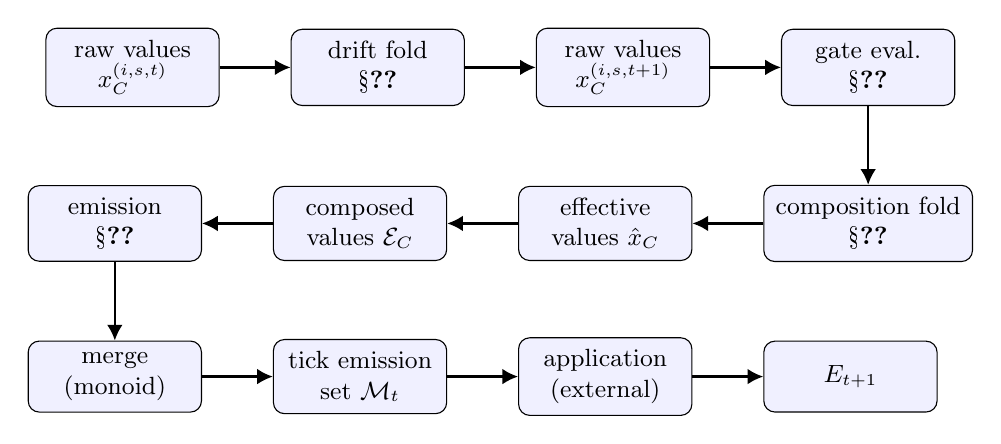
\begin{tikzpicture}[node distance=10mm and 9mm]
  \node[block] (s1) {raw values\\$x_C^{(i,s,t)}$};
  \node[block, right=of s1] (drift) {drift fold\\\S\ref{sec:drift}};
  \node[block, right=of drift] (s2) {raw values\\$x_C^{(i,s,t+1)}$};
  \node[block, right=of s2] (gate) {gate eval.\\\S\ref{sec:gates}};

  \node[block, below=of gate] (compose) {composition fold\\\S\ref{sec:compose}};
  \node[block, left=of compose] (eff) {effective\\values $\hat{x}_C$};
  \node[block, left=of eff] (cv) {composed\\values $\mathcal{E}_C$};
  \node[block, left=of cv] (em) {emission\\\S\ref{sec:emit}};

  \node[block, below=of em] (merge) {merge\\(monoid)};
  \node[block, right=of merge] (M) {tick emission\\set $\mathcal{M}_t$};
  \node[block, right=of M] (apply) {application\\(external)};
  \node[block, right=of apply] (env) {$E_{t+1}$};

  \draw[arrow] (s1) -- (drift);
  \draw[arrow] (drift) -- (s2);
  \draw[arrow] (s2) -- (gate);
  \draw[arrow] (gate) -- (compose);
  \draw[arrow] (compose) -- (eff);
  \draw[arrow] (eff) -- (cv);
  \draw[arrow] (cv) -- (em);
  \draw[arrow] (em) -- (merge);
  \draw[arrow] (merge) -- (M);
  \draw[arrow] (M) -- (apply);
  \draw[arrow] (apply) -- (env);
\end{tikzpicture}
\caption{The per-tick state-transition operator. Boxes are pure functions; arrows are data dependencies. Application is the only step that writes world variables, and it lies outside the model.}
\label{fig:tick}
\end{figure}

% =========================================================================
\section{Runtime Vocabulary Genesis}
\label{sec:genesis}

The objects of \cref{sec:channels,sec:state,sec:gates,sec:compose,sec:drift,sec:emit} form a fixed vocabulary: the registries $\mathcal{B}, \mathcal{C}, \mathcal{V}, \mathcal{P}$ and the kind sets for gates and drift. We now relax the assumption that this vocabulary is fixed and define a transition that may extend it between ticks. The intent is to model open-ended simulations in the sense of Soros and Stanley~\cite{soros2014}: the model's expressive ceiling rises with its history.

\notationtable{Symbols introduced in \cref{sec:genesis} (excluding revision; see \cref{sec:revision}).}{tab:notation-genesis}{
$\mathcal{R}_t$           & 7-tuple                      & registry tuple at tick $t$ \\
$\bar{\mathcal{G}}$       & set, frozen                  & gate-kind registry \\
$\bar{\mathcal{D}}$       & set, frozen                  & drift-kind registry \\
$L_t$                     & finite sequence              & lineage event log up to tick $t$ \\
$\mathcal{G}_t$           & function                     & genesis transition operator \\
$T_G$                     & $\mathbb{N}$                 & genesis cadence \\
$g$                       & tuple                        & a genesis event \\
$\mathrm{id}_g, t_g$      & $\mathbb{I}, \mathbb{N}$     & event identifier and tick \\
$\kappa_g$                & kind tag                     & channel-kind tag (channel, primitive, etc.) \\
$n_g$                     & $\mathbb{I}$                 & new identifier created by event \\
$\mathfrak{m}_g$          & $\{\mathrm{Cmp},\mathrm{Lat},\mathrm{Mut}\}$ & mechanism (composition / latent extraction / mutation) \\
$\mathrm{par}_g$          & $\subset \mathcal{C}_{t_g - 1}$ & parent channel set \\
$\omega_g$                & $\mathbb{I}$                 & source-population identifier \\
$q_g$                     & $\mathbb{R}_{\ge 0}$         & event's fitness witness \\
$a$                       & ---                          & an agent \\
$\rho_a^t$                & $\mathbb{R}$                 & agent $a$'s residual at tick $t$ (novelty signal) \\
$\mathfrak{B}_a$          & finite set                   & latent slot buffer of agent $a$ \\
$j$                       & $\mathbb{N}$                 & slot index \\
$\mathbf{u}_j$            & $\mathbb{R}^{|\mathcal{C}_{t-1}|}$ & sparse signature vector of slot $j$ \\
$w_j$                     & $\mathbb{R}_{\ge 0}$         & slot weight \\
$t_j$                     & $\mathbb{N}$                 & last-touched tick of slot $j$ \\
$K_a$                     & $\mathbb{N}$                 & bound on $|\mathfrak{B}_a|$ \\
$j(\rho)$                 & $\mathbb{N}$                 & slot-lookup function for residual $\rho$ \\
$W_t$                     & aggregate                    & population-level state used by genesis \\
$\beta$                   & finite set of agents         & a candidate bucket \\
$n_{\min}$                & $\mathbb{N}$                 & bucket-eligibility threshold \\
$\Omega_\kappa$           & set                          & registered composition operators for kind $\kappa$ \\
$\kappa$                  & kind tag                     & channel kind in the genesis context \\
$A$                       & $\subseteq \mathcal{C}_{t-1}$ & parent subset for composition \\
$\omega$                  & $\Omega_\kappa$              & a composition operator instance \\
$C_\beta^{\mathrm{Cmp}}, C_\beta^{\mathrm{Lat}}, C_\beta^{\mathrm{Mut}}$ & candidates & per-mechanism proposals for bucket $\beta$ \\
$C_\beta^*$               & candidate                    & winner, $\arg\max$ over the three mechanisms \\
$q$                       & function                     & fitness function: variance in residuals explained \\
$q_{\min}$                & $\mathbb{R}_{\ge 0}$         & admission threshold \\
$N_\kappa, K_\kappa$      & $\mathbb{N}$                 & niche granularity and per-niche cap for kind $\kappa$ \\
$H$                       & function                     & deterministic hash function \\
$A_C^t$                   & $\mathbb{R}_{\ge 0}$         & activity score of $C$ at tick $t$ \\
$\lambda_g$               & $[0,1]$                      & per-cadence activity decay rate \\
$A_{\min}$                & $\mathbb{R}_{\ge 0}$         & retire threshold \\
$\mathrm{usage}(C, t)$    & $\mathbb{R}_{\ge 0}$         & instantaneous usage of $C$ at tick $t$ \\
$d$                       & metric                       & signature distance metric \\
$\mathrm{cov}_{a \in \beta}$ & matrix                    & empirical covariance over the agents of bucket $\beta$ \\
$\mathrm{perturb}(\cdot, \omega)$ & function              & mutation perturbation under PRNG stream $\omega$ \\
}

\subsection{Provenance}

Provenance is a string-valued tag matching the regular language
\[
\Pi \;=\; \mathtt{core} \;\big|\; \mathtt{mod}\!:\!\mathbb{I} \;\big|\; \mathtt{genesis}\!:\!\mathbb{I}\!:\!\mathbb{N}\!:\!\mathbb{I}\!:\!\mathbb{I}
\]
where the four-component genesis form encodes a source population, a tick of birth, a kind tag, and a deterministic hash. \Cref{sec:revision} extends this language with a fifth alternative for revision events.

\subsection{The Registry Tuple and Lineage Log}

Let $\mathcal{R}_t$ denote the tuple
\[
\mathcal{R}_t \;=\; \langle\, \mathcal{B},\; \bar{\mathcal{G}},\; \bar{\mathcal{D}},\; \mathcal{V}_t,\; \mathcal{C}_t,\; \mathcal{P}_t,\; L_t \,\rangle
\]
where $\bar{\mathcal{G}}, \bar{\mathcal{D}}$ are the gate-kind and drift-kind registries (held fixed) and $L_t$ is an append-only finite sequence of \emph{lineage events}.

When the channel registry grows at runtime, \emph{something} has to record what was added, why, and from which parents. A genesis event is that record: a tick stamp, a mechanism, a parent set, a fitness witness. It is enough to replay the addition deterministically, and enough to trace any descendant channel back to its seeds.

\begin{definition}[Genesis event]
A genesis event is
\[
g \;=\; \langle\, \mathrm{id}_g,\; t_g,\; \kappa_g,\; n_g,\; \mathfrak{m}_g,\; \mathrm{par}_g,\; \omega_g,\; q_g \,\rangle
\]
where $\kappa_g$ is the kind tag (channel, primitive, etc.); $n_g \in \mathbb{I}$ is the new id; $\mathfrak{m}_g \in \{\mathrm{Cmp},\mathrm{Lat},\mathrm{Mut}\}$ is the mechanism (composition, latent extraction, mutation); $\mathrm{par}_g \subset \mathcal{C}_{t_g - 1}$ is the parent set, possibly empty for $\mathrm{Lat}$; $\omega_g \in \mathbb{I}$ is the source-population identifier; and $q_g \in \mathbb{R}_{\ge 0}$ is the candidate's fitness.
\end{definition}

\subsection{The Novelty Signal}

Each agent $a$ in the simulation produces a per-tick \emph{residual} $\rho_a^t \in \mathbb{R}$ measuring the part of its observed behaviour unexplained by the current channel set. The model is agnostic to how $\rho$ is computed; in active-inference settings~\cite{friston2010} it is the log-density gap between the empirical action distribution and the EFE-optimal one, but any divergence-style novelty signal will do, including the spin-off statistics of Drescher's schema mechanism~\cite{drescher1991}.

Each agent maintains a bounded latent-slot buffer
\[
\mathfrak{B}_a \;=\; \bigl\{(j,\, \mathbf{u}_j,\, w_j,\, t_j)\bigr\}_{j=1}^{K_a}
\]
where $\mathbf{u}_j \in \mathbb{R}^{|\mathcal{C}_{t-1}|}$ is a sparse signature vector over existing channels, $w_j \in \mathbb{R}_{\ge 0}$ an accumulated weight, and $K_a$ a bound. The per-tick update is
\[
w_{j(\rho_a^t)} \;\leftarrow\; w_{j(\rho_a^t)} + |\rho_a^t|, \qquad t_{j(\rho_a^t)} \leftarrow t,
\]
where $j(\rho)$ is the slot whose signature is closest to the residual's projection (with insertion of a new slot when no slot is sufficiently close); eviction when $|\mathfrak{B}_a| > K_a$ is by stable lexicographic sort on $(w, t, j)$.

\subsection{The Genesis Transition}
\label{sec:gtrans}

The genesis transition is the operator that may grow the registry. We do not run it every tick: registry changes are expensive (every shard must learn about them) and the latent-pressure signal needs time to accumulate before it can support stable clustering. Instead, the transition runs once every $T_G$ ticks, the \emph{genesis cadence}, and is the identity at every other tick. When it does run, it executes the four-step pipeline of bucket clustering, candidate proposal, admission, and registration described below.

The genesis transition is a stride-$T$ operator with stride $T = T_G$ (the \emph{genesis cadence}):
\[
\mathcal{G}_t \;:\; (\mathcal{R}_{t-1},\, W_{t-1}) \;\longmapsto\; (\mathcal{R}_t,\, W_t),
\]
where $W$ aggregates the buffers $\{\mathfrak{B}_a\}$ and the population structure. When $t \not\equiv 0 \pmod T$, $\mathcal{G}_t$ is the identity. Otherwise the transition is the composition of four steps.

\paragraph{Step 1: bucket clustering.} Partition the agent population into buckets by signature similarity; each bucket $\beta$ contains agents whose top latent slot is close in $\mathbf{u}$. A bucket is \emph{eligible} if $|\beta| \ge n_{\min}$.

\paragraph{Step 2: candidate proposal.} For each eligible bucket $\beta$ and channel kind $\kappa$, three candidate channels are constructed in parallel.

\emph{Composition} draws from a registered set $\Omega_\kappa$ of operators~\cite{arthur2009,lake2015} over subsets of existing channels:
\[
C_\beta^{\mathrm{Cmp}} \;=\; \arg\max_{(\omega, A) \in \Omega_\kappa \times 2^{\mathcal{C}_{t-1}}}\, q\bigl(\omega(A),\, \beta\bigr).
\]
\emph{Latent extraction} takes the top eigenvector of the within-bucket covariance of slot signatures (an Indian-buffet-process-style step~\cite{griffiths2011}):
\[
C_\beta^{\mathrm{Lat}} \;=\; \mathrm{top\,eigenvector}\!\bigl(\mathrm{cov}_{a \in \beta}\, \mathbf{u}_a\bigr).
\]
\emph{Mutation} perturbs the parameters of the channel nearest to $\beta$'s mean signature:
\[
C_\beta^{\mathrm{Mut}} \;=\; \mathrm{perturb}\!\bigl(\arg\min_{C \in \mathcal{C}_{t-1}} d(\mathbf{u}_\beta, \mathbf{u}_C),\, \omega\bigr).
\]
The fitness $q$ measures how much variance in $\beta$'s residuals the candidate explains. The bucket's winner is
\[
C_\beta^* \;=\; \arg\max_{\mathfrak{m} \in \{\mathrm{Cmp},\mathrm{Lat},\mathrm{Mut}\}}\, q\bigl(C_\beta^\mathfrak{m},\, \beta\bigr).
\]

\paragraph{Step 3: admission.} A quality--diversity archive~\cite{lehman2011,mouret2015} partitions the candidate space into niches; admission is per-niche dominance. Admitted iff $q(C_\beta^*) \ge q_{\min}$ and $C_\beta^*$ dominates an incumbent of its niche or fills an empty niche slot. The bound on archive size is
\[
|\mathcal{C}_t^{\mathrm{genesis}}| \;\le\; \sum_\kappa N_\kappa \cdot K_\kappa,
\]
ensuring the registry stays finite for any simulation length. The dominated-novelty admission criterion of~\cite{lim2025} is a refinement compatible with this bound.

\paragraph{Step 4: registration and bookkeeping.} For each admitted $C_\beta^*$:
\begin{align*}
n &= \mathtt{genesis}\!:\!\omega_\beta\!:\!t\!:\!\kappa\!:\!H\!\bigl(\mathbf{u}_\beta,\, \mathrm{sort}(\mathrm{par}),\, \mathfrak{m}\bigr),\\
\pi_{C_\beta^*} &= n,\\
\mathcal{C}_t &\leftarrow \mathcal{C}_{t-1} \cup \{C_\beta^*\},\\
L_t &\leftarrow L_{t-1} \cdot g_\beta,
\end{align*}
where $H$ is a deterministic hash. Garbage collection retires channels whose evolutionary-activity score~\cite{bedau1998}
\[
A_C^t \;=\; (1 - \lambda_g)\, A_C^{t-1} \;+\; \mathrm{usage}(C, t)
\]
falls below $A_{\min}$; retired channels leave $\mathcal{C}_t$ but their entries in $L$ are preserved.

In plain English, the pipeline does the following. Look across the population for clusters of agents whose unmodelled-behaviour signatures agree (Step 1). For each such cluster, propose three candidate new channels by three different routes: one by combining existing channels (Step 2, Composition), one by extracting a new latent direction from the residuals of the cluster (Step 2, Latent extraction), and one by perturbing the existing channel that is closest to the cluster's signature (Step 2, Mutation). Pick the candidate that explains the cluster's residuals best, admit it only if it dominates the relevant niche of an archive (Step 3), and record it with a hash-based identifier and a lineage entry (Step 4). Channels that stop being used decay out of the registry on their own.

\subsection{Diagram of the Genesis Pipeline}

\Cref{fig:genesis} shows the dataflow.

\begin{figure}[ht]
\centering
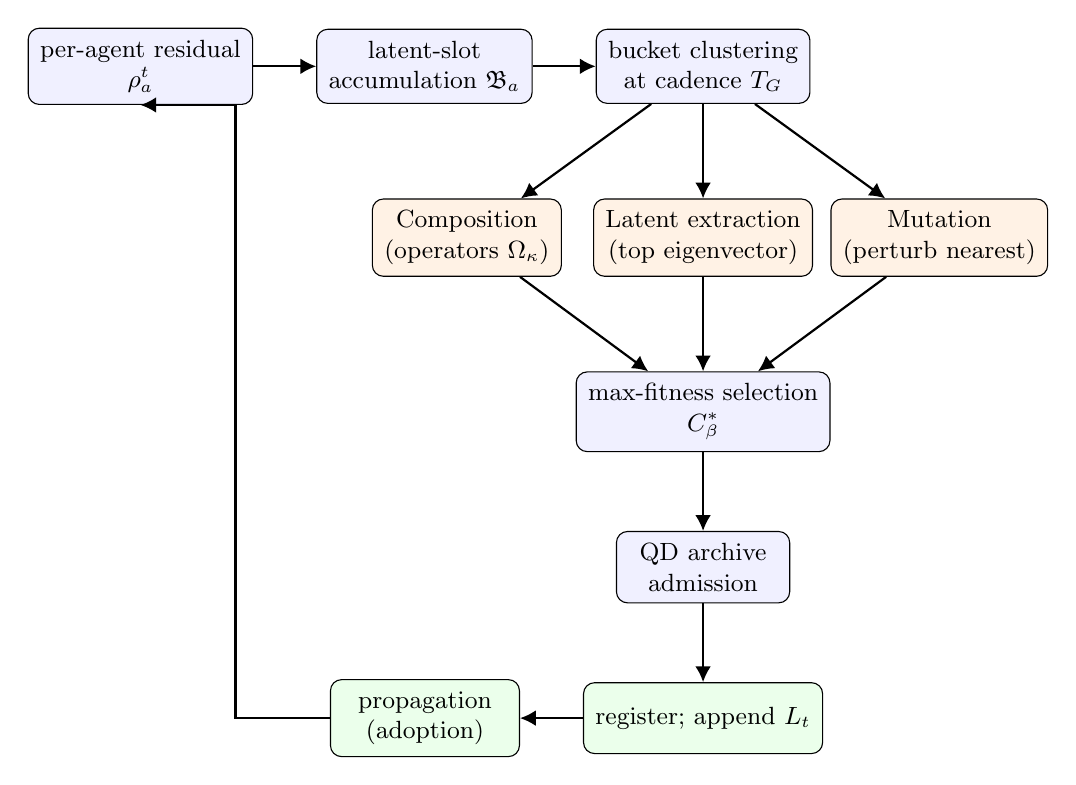
\begin{tikzpicture}[node distance=10mm and 8mm]
  \node[block] (rho) {per-agent residual\\$\rho_a^t$};
  \node[block, right=of rho] (slot) {latent-slot\\accumulation $\mathfrak{B}_a$};
  \node[block, right=of slot] (clust) {bucket clustering\\at cadence $T_G$};

  \node[branchblock, below=12mm of clust, xshift=-30mm] (cmp) {Composition\\(operators $\Omega_\kappa$)};
  \node[branchblock, below=12mm of clust] (lat) {Latent extraction\\(top eigenvector)};
  \node[branchblock, below=12mm of clust, xshift=30mm] (mut) {Mutation\\(perturb nearest)};

  \node[block, below=12mm of lat] (pick) {max-fitness selection\\$C_\beta^*$};
  \node[block, below=of pick] (qd) {QD archive\\admission};
  \node[endblock, below=of qd] (reg) {register; append $L_t$};
  \node[endblock, left=of reg] (prop) {propagation\\(adoption)};

  \draw[arrow] (rho) -- (slot);
  \draw[arrow] (slot) -- (clust);
  \draw[arrow] (clust) -- (cmp);
  \draw[arrow] (clust) -- (lat);
  \draw[arrow] (clust) -- (mut);
  \draw[arrow] (cmp) -- (pick);
  \draw[arrow] (lat) -- (pick);
  \draw[arrow] (mut) -- (pick);
  \draw[arrow] (pick) -- (qd);
  \draw[arrow] (qd) -- (reg);
  \draw[arrow] (reg) -- (prop);
  \draw[arrow] (prop.west) -- ++(-12mm,0) |- (rho.south);
\end{tikzpicture}
\caption{The genesis pipeline. Three proposal mechanisms run in parallel; the maximum-fitness candidate is admitted iff it dominates an incumbent in its quality--diversity niche. Adoption events feed back into agent residuals on the next tick.}
\label{fig:genesis}
\end{figure}

\subsection{Closure Properties}

The next theorem is the model's load-bearing closure property. It says: even though the channel registry can grow without bound at runtime, every channel in it can be traced back to an original seed (kernel or mod) through finitely many recorded events. This is what gives the model its replay guarantee even in the open-ended setting --- a save file plus the global seed and the lineage log is enough to reconstruct the registry at any tick.

\begin{theorem}[Lineage closure]\label{thm:lineage}
For every $C \in \mathcal{C}_t$ with $\pi_C$ matching the genesis pattern, there is a finite path
\[
C \;=\; C_n \to C_{n-1} \to \cdots \to C_0
\]
in the partial order \emph{parent-of (in $L_t$)} such that $\pi_{C_0} \in \{\mathtt{core}\} \cup \{\mathtt{mod}\!:\!m \mid m \in \mathbb{I}\}$.
\end{theorem}

\begin{proof}
By induction on the tick at which $C$ was registered. If $C$ was registered at tick $t' \le t$, then $L_{t'}$ contains an event $g$ with $n_g = \mathrm{id}_C$ and $\mathrm{par}_g \subseteq \mathcal{C}_{t'-1}$; for the $\mathrm{Lat}$ mechanism, $\mathrm{par}_g$ is replaced by the support set of agents whose signatures are themselves indexed over $\mathcal{C}_{t'-1}$. Either way, every parent's provenance is non-genesis (in which case the path terminates) or itself a genesis entry registered strictly earlier, where the inductive hypothesis applies.
\end{proof}

The closure theorem shows the registry is traceable; the next lemma shows it does not grow unboundedly. The two together give us a registry that is both open-ended (new entries can always appear) and bounded (the total active count is capped).

\begin{lemma}[Bounded vocabulary]\label{lem:bounded}
Under the quality--diversity admission rule with niche granularities $N_\kappa$ and per-niche caps $K_\kappa$,
\[
|\mathcal{C}_t \setminus \mathcal{C}_0| \;\le\; \sum_\kappa N_\kappa K_\kappa
\]
for all $t$.
\end{lemma}

\begin{proof}
Admission of a new entry into a saturated niche requires retirement of an incumbent; non-saturated niches are bounded by $K_\kappa$ each.
\end{proof}

\subsection{Retrospective Revision}
\label{sec:revision}

The genesis transition can register new channels but cannot redefine existing ones. Cultural-evolutionary systems regularly do redefine: a word's referent shifts, a tool's purpose drifts, an ideology fissions into rival sects. The challenge is to admit such redefinition without violating \cref{thm:lineage}, which depends on every channel having a lineage chain to a fixed seed set.

\notationtable{Symbols introduced in \cref{sec:revision}.}{tab:notation-revision}{
$\mathcal{V}_t^{\mathrm{rev}}$ & function               & revision transition operator \\
$r$                       & tuple                        & a revision event (overloads $r$ as running value in $\eta_\kappa$) \\
$\mathrm{id}_r, t_r$      & $\mathbb{I}, \mathbb{N}$     & event identifier and tick \\
$C_r^{\mathrm{prev}}$     & $\mathcal{C}_{t_r - 1}$      & parent channel \\
$C_r^{\mathrm{next}}$     & fresh channel                & child channel \\
$\mathrm{policy}_r$       & $\{\mathrm{deprecate}, \mathrm{coexist}\}$ & post-revision parent policy \\
$\Delta_r$                & $\mathbb{R}_{\ge 0}$         & semantic-distance witness (overloads drift list $\Delta_C$) \\
$\Pi'$                    & $\Pi \cup \dots$             & provenance grammar extended for revisions \\
$\gamma_\bot$             & gate instance                & synthetic always-fail gate (used by deprecation) \\
$\Delta_{\mathrm{rev}}$   & $\mathbb{R}_{\ge 0}$         & threshold above which a Mutation candidate is reclassified as a revision \\
}

We extend the lineage log $L_t$ with a second class of events. A revision event creates a fresh channel from a single parent and optionally silences the parent. The core ideas are: (i) a revised channel is a \emph{new} entry in $\mathcal{C}_t$, not an in-place mutation of an existing one (so channel-id immutability is preserved); (ii) the parent--child edge appears explicitly in $L_t$ (so \cref{thm:lineage} extends by induction); (iii) the parent's deprecation is implemented as an additional gate, not a deletion (so the composition fold retains its totality property).

A revision event is the formal record of ``what looked like a drifted channel should actually be treated as a new channel that supersedes the old one.'' In a cultural-evolutionary setting this happens constantly: words shift meaning, tools evolve to do something new, ideologies fork. The event records a parent, a child that supersedes it, a policy ($\mathrm{deprecate}$ silences the parent; $\mathrm{coexist}$ keeps it alive alongside), and a witness for how far the new meaning is from the old.

\begin{definition}[Revision event]\label{def:revision}
A revision event at tick $t_r$ is a tuple
\[
r \;=\; \langle\, \mathrm{id}_r,\; t_r,\; C_r^{\mathrm{prev}},\; C_r^{\mathrm{next}},\; \mathrm{policy}_r,\; \Delta_r \,\rangle
\]
where $C_r^{\mathrm{prev}} \in \mathcal{C}_{t_r-1}$, $C_r^{\mathrm{next}} \notin \mathcal{C}_{t_r-1}$, $\mathrm{policy}_r \in \{\mathrm{deprecate},\mathrm{coexist}\}$, and $\Delta_r \in \mathbb{R}_{\ge 0}$ is a semantic-distance witness (the magnitude by which $C_r^{\mathrm{next}}$ diverges from $C_r^{\mathrm{prev}}$ in some chosen metric; we leave the metric abstract).
\end{definition}

The new channel's identifier encodes its parent's identifier, the tick of revision, and a hash of the distance witness. Just by looking at a channel id, you can see whether it is a revision and what it revises --- which is what makes the lineage edge ``inspectable from the identifier alone.''

\begin{definition}[Revision identifier]\label{def:revid}
The provenance language $\Pi$ is extended to
\[
\Pi' \;=\; \Pi \;\cup\; \{\mathtt{revision}\!:\!\mathbb{I}\!:\!\mathbb{N}\!:\!\mathbb{I}\}
\]
and the new channel's identifier is
\[
\mathrm{id}(C_r^{\mathrm{next}}) \;=\; \mathtt{revision}\!:\!\mathrm{id}(C_r^{\mathrm{prev}})\!:\!t_r\!:\!H(\Delta_r,\, \mathrm{id}_r).
\]
The first component is the parent's id, making the lineage edge inspectable from the identifier alone.
\end{definition}

The transition itself appends to the registry and the lineage log, exactly like genesis. The only new wrinkle is the deprecation policy: under $\mathrm{deprecate}$, the parent gets a synthetic always-fail gate, which makes its effective value zero forever after; under $\mathrm{coexist}$, the parent is left untouched and both channels live on. The two policies model two recognisable cultural-evolutionary processes: linguistic semantic shift on one hand, sectarian schism on the other.

\begin{definition}[Revision transition]\label{def:revtrans}
The revision transition $\mathcal{V}_t^{\mathrm{rev}}$ runs at the same cadence as $\mathcal{G}_t$ and is composed with it. For each admitted revision event $r$ at tick $t$:
\begin{align*}
\mathcal{C}_t &\leftarrow \mathcal{C}_{t-1} \cup \{C_r^{\mathrm{next}}\}, \\
L_t &\leftarrow L_{t-1} \cdot r, \\
\Gamma_{C_r^{\mathrm{prev}}} &\leftarrow
\begin{cases}
\Gamma_{C_r^{\mathrm{prev}}} \cup \{\gamma_\bot\} & \text{if } \mathrm{policy}_r = \mathrm{deprecate}, \\
\Gamma_{C_r^{\mathrm{prev}}} & \text{if } \mathrm{policy}_r = \mathrm{coexist},
\end{cases}
\end{align*}
where $\gamma_\bot$ is a synthetic gate instance whose predicate is the constant $0$. Under the deprecate policy, $\Phi_{C_r^{\mathrm{prev}}} \equiv 0$ at tick $t+1$ and onward by \cref{def:effective}; the parent's raw value is preserved (for save-compatibility and replay) but its effective contribution to all downstream composition and emission is silenced. Under the coexist policy, both channels remain active and their fates are independently decided by garbage collection.
\end{definition}

\paragraph{When does revision fire?} Revision events are not a fourth proposal mechanism; they are a re-classification of the Mutation candidates from \cref{sec:gtrans} step~2. When a Mutation candidate's distance from its parent exceeds a threshold $\Delta_{\mathrm{rev}}$, the engine emits a revision event with $C_r^{\mathrm{next}}$ set to the candidate, $C_r^{\mathrm{prev}}$ to the parent, and $\Delta_r$ to the witnessed distance. The default policy is $\mathrm{deprecate}$; $\mathrm{coexist}$ is selected when the bucket of supporting agents is itself bimodal in $\mathbf{u}$, i.e.\ when two sub-populations want the parent to mean two different things. This reclassification leaves the per-tick cost unchanged.

The closure theorem from earlier extends to revisions because every revision edge, like every genesis edge, points backward in tick order. Strong induction does the rest --- the lineage forest is finite-depth no matter how deeply the registry has been revised.

\begin{theorem}[Lineage closure under revision]\label{thm:lineage-rev}
Augment the parent-of relation in $L_t$ with revision edges $C_r^{\mathrm{next}} \to C_r^{\mathrm{prev}}$ for every revision event $r$. Then for every $C \in \mathcal{C}_t$ with $\pi_C \in \Pi'$, there is a finite path under the augmented relation to a non-genesis-non-revision seed.
\end{theorem}

\begin{proof}
Strong induction on the tick of registration. Every revision edge points from a tick-$t_r$ child to a tick-$(t_r-1)$-or-earlier parent in $\mathcal{C}_{t_r-1}$; every genesis edge does likewise. The augmented relation therefore strictly decreases tick along edges, so chains are finite, and each finite chain terminates at a node with provenance in $\{\mathtt{core}\} \cup \{\mathtt{mod}\!:\!m\}$.
\end{proof}

The next lemma is partly a sanity check: under genesis-and-revision combined, the lineage forest can grow in three ways, and these three ways exhaust the elementary local operations on a forest whose edges respect tick order. So we have not accidentally left out a topological possibility.

\begin{lemma}[Topological moves on the lineage forest]\label{lem:moves}
Together, the genesis transition and the revision transition support three nontrivial topological operations on the lineage forest, summarised in \cref{tab:moves}. Under the constraint that no edge in $L_t$ may point backward in tick order, these moves are exhaustive of the elementary local operations on a labelled forest.
\end{lemma}

\begin{table}[ht]
\centering
\caption{The three nontrivial moves on the lineage forest, as realised by the genesis and revision transitions.}
\label{tab:moves}
\small
\begin{tabularx}{\linewidth}{l L{0.40\linewidth} L{0.30\linewidth}}
\toprule
Move & Topological action & Realised by \\
\midrule
Fusion             & two parents $\to$ one child                                       & genesis-by-Composition (\cref{sec:gtrans} step 2) \\
Fissioning         & one parent $\to$ multiple children, all live                       & two or more revision events with $\mathrm{policy} = \mathrm{coexist}$ sharing a parent \\
Semantic shift     & one parent $\to$ one child, parent silenced                        & revision with $\mathrm{policy} = \mathrm{deprecate}$ \\
\bottomrule
\end{tabularx}
\end{table}

\paragraph{Bounded growth.} The vocabulary bound of \cref{lem:bounded} extends to the joint genesis-and-revision system if revision children are charged to the same quality--diversity niches as their parents. The deprecation gate is a per-channel state, not a registry entry, and so does not consume archive slots; under the deprecate policy, revision is approximately registry-conservative (the deprecated parent stays in $\mathcal{C}_t$ but contributes nothing to active channel use, and is collected by the activity-score garbage collector once usage decays). Under the coexist policy, both channels compete for the same niche slots.

\paragraph{Fusion.} The dual operation --- two parents producing one revised child --- is what genesis-by-Composition already does. So fusion is genesis-by-Composition; fissioning is revision-by-coexist; semantic-shift-with-deprecation is revision-by-deprecate. The three nontrivial topological moves on a labelled forest are jointly covered.

\paragraph{Why not in-place semantic shift?} A simpler-looking design would let an existing channel's parameters drift over time, with no new identifier. We rejected this: channel-id immutability is what gives save files and replay journals their stability across the simulation's runtime. A reference to channel $C$ written into a save at tick $t_1$ and read at tick $t_2 > t_1$ must mean the same thing at both ticks; in-place semantic shift breaks this. Branching lineage with deprecation gives the same expressive power at the cost of one additional registry entry per redefinition --- a price that \cref{lem:bounded} bounds globally.

% =========================================================================
\section{Properties}
\label{sec:properties}

We collect the structural properties the model satisfies by construction.

\paragraph{Determinism.} $\mathcal{T}$, $\mathcal{G}$, and $\mathcal{V}^{\mathrm{rev}}$ are deterministic functions of their inputs and of the threaded pseudorandom states. The proof obligations are (i) every fold is over a sorted list with a total operator (\cref{lem:comp-det,lem:drift-range}), (ii) every reduction over instances is over a commutative monoid (\cref{lem:merge-comm}), (iii) every random draw is from a named seeded stream (\cref{sec:drift}).

\paragraph{Registry monolithicism.} There is a single registry per kind, queried by all simulation systems uniformly; no system holds a private list of channel ids. Genesis appends to the channel registry. Revision also appends; it never deletes or rewrites. The deprecation policy of \cref{def:revtrans} is implemented as a gate annotation on the parent, not as removal.

\paragraph{Emergence closure.} Every change to a world variable traces to a primitive emission (\cref{def:emission}); every primitive emission traces to a composition hook on a channel; every channel is in $\mathcal{C}_t$; every entry of $\mathcal{C}_t$ is either a seed or, by \cref{thm:lineage,thm:lineage-rev}, traces to seeds through finitely many recorded events. There are no mechanisms outside this chain.

\paragraph{Mechanics--label separation.} The operators $\eta_\kappa$, predicates $\phi_{\bar{g}}$, and drift functions $f_{\bar{d}}$ branch only on kind tags, never on channel ids or names. Names exist only as keys into the registries. Any naming the simulation acquires is the work of an external process --- a labeller observing emission patterns over time --- and not of the kernel.

% =========================================================================
\section{Design Rationale}
\label{sec:rationale}

The shape of the model reflects a small number of considered choices, summarised in \cref{tab:rationale}.

\begin{longtable}{L{0.25\textwidth} L{0.25\textwidth} L{0.40\textwidth}}
\caption{Design choices and the reasoning behind them.}
\label{tab:rationale}\\
\toprule
Choice & Alternatives & Rationale \\
\midrule
\endfirsthead
\multicolumn{3}{c}{\tablename\ \thetable{} (continued)}\\
\toprule
Choice & Alternatives & Rationale \\
\midrule
\endhead
\bottomrule
\endfoot
Channel as a real-valued scalar with a range
& Vector channels; categorical channels; channels with dynamic ranges
& The scalar-with-range form is the smallest abstraction closed under the operator set; it admits the gene-regulatory-network reading~\cite{wagner2011} and the gameplay-attribute reading~\cite{stanley2007}, unifying biological and engineered substrates. Vector channels balloon the operator vocabulary; categoricals break drift; dynamic ranges break replay. \\
Carrier as the only grouping over channels
& A pre-imposed taxonomy (sensory, motor, \ldots); free-form tags; no grouping
& Carriers correspond to dynamical regimes (mutation in genomes, wear in artefacts, institutional drift in collectives), not to semantic categories. Making the only grouping structural avoids prematurely classifying behaviour and keeps the model neutral across substrates. \\
Drift before composition
& Composition reads stale raw and writes back; interleaved
& Sequencing drift then composition keeps each $C$ singly-valued per tick; replays are trivial; no information leaks across the boundary. \\
Dormant channel contributes effective $0$
& Skip the channel; raise an exception
& Sending dormant channels to $0$ makes every operator total. Composition is a left fold over a list of partial functions if dormant channels are removed, but a left fold over a list of total functions if they evaluate to $0$. Totality is worth more than terseness. \\
Sorted-by-id composition fold
& Parallel reduction; insertion-order fold
& The composition operators are non-commutative ($\eta_{\mathrm{mul}}$ followed by $\eta_{\mathrm{thr}}$ differs from the reverse). A fixed deterministic order is required; sort-by-id is the cheapest such order. \\
Merge restricted to commutative monoids
& First-emitter-wins; ordered weighted; arbitrary
& \cref{lem:merge-comm} fails without commutativity; replays then depend on iteration order, which depends on hash-table seeds, which destroys the determinism guarantee. \\
Carrier-scoped channel ids
& Globally unique ids
& Scoping permits the same channel name to mean different things on different carriers (e.g.\ \emph{durability} on artefacts and on settlements) without name collision; the registry is keyed by the pair, the model treats the pair as primitive. \\
Genesis as registry append with a lineage log
& Fork-and-replace; in-place mutation; copy-on-write
& Append plus garbage collection keeps the lineage in $L_t$ permanently and leaves seeds immutable, satisfying \cref{thm:lineage}. The other options either lose lineage or break monolithicism. \\
Genesis identifiers encode parents and signature hash
& Random UUIDs; sequential counters
& Hash-based identifiers allow deterministic replay and preserve traceability without an external lookup. Sequential counters collide across forked replays. \\
Three genesis mechanisms in parallel
& Any single mechanism alone
& Each mechanism reaches different parts of channel space: composition explores combinatorial closure~\cite{arthur2009}; latent extraction discovers principal directions in residual covariance~\cite{griffiths2011}; mutation provides local search. The Soros--Stanley~\cite{soros2014} necessary conditions are simultaneously satisfied only when reproduction, novelty, and selection are all present. \\
Quality--diversity archive admission
& No admission rule (unbounded growth); global fitness; time-based eviction
& \cref{lem:bounded} fails without a per-niche cap; global-fitness admission collapses diversity~\cite{lehman2011}; time-based eviction discards channels that are durably useful. The dominated-novelty variant of~\cite{lim2025} gives the cleanest stationary distribution. \\
Revision via branching lineage with gate-deprecation
& In-place semantic shift over a fixed id; fork-and-replace; no revision
& Preserves \cref{thm:lineage,thm:lineage-rev} by treating revision as a labelled edge in $L_t$. In-place semantic shift directly violates channel-id immutability, breaking save-compatibility; fork-and-replace loses lineage; no-revision rules out the most common mode of cultural change. \\
Revision triggered by Mutation-distance threshold
& Independent revision proposal mechanism; player- or designer-triggered only; revision-on-every-mutation
& Reuses existing proposal machinery, so the per-tick cost of revision is zero. The threshold $\Delta_{\mathrm{rev}}$ is a single scalar parameter; revision-on-every-mutation collapses fissioning into ordinary mutation drift. \\
Coexist policy uses bucket bimodality as the trigger
& Always coexist; always deprecate; user-specified per event
& Bimodality of the supporting bucket is the diagnostic that two sub-populations want the parent to mean different things. Without it, fissioning would create channels with no support population. With it, fissioning is the natural model of sectarian schism. \\
\end{longtable}

% =========================================================================
\section{Open Questions}
\label{sec:open}

Three questions seem to most deserve attention.

The first concerns the \emph{fitness} function $q$ in \cref{sec:gtrans}. We have specified it abstractly as ``variance in residuals explained''; concrete instantiations differ in how they weight short-lived vs.\ long-lived novelty. The choice has measurable consequences for the steady-state vocabulary's richness and for whether genesis converges or persistently churns.

The second concerns the \emph{semantic-distance metric} underlying $\Delta_r$ in \cref{def:revision}. We have left it abstract; candidate choices include cosine distance over signature vectors, Kullback--Leibler divergence over induced action distributions, and Wasserstein distance over the candidate's emission distribution against the parent's. The metric controls how readily revision fires versus how readily ordinary Mutation fires; fixing it well is empirical, but the model is robust to which choice is made provided the metric is symmetric and continuous.

The third is the absence of a notion of \emph{ancestor reactivation}: a deprecated channel cannot be ``rehabilitated'' without going through a fresh revision event. Cultural-evolutionary systems sometimes exhibit such reactivation (a deprecated practice returns under its old name centuries later). Modelling it cleanly would require either a second category of policy ($\mathrm{rehydrate}$) on revision events with the parent itself as the child, or a relaxation of the revision-event identifier to refer to a sub-history of $L$ --- both speculative. A natural starting point is the hierarchical Indian-buffet construction of Lijoi et al.~\cite{lijoi2023}, which provides priors over feature reuse across populations.

% =========================================================================
\appendices

\section{Distributed Implementation: Sharded Lineage with Deterministic Merge}
\label{appx:sldm}

The model of \cref{sec:tick,sec:genesis,sec:revision} is defined abstractly. This appendix sketches a concrete implementation, which we call \emph{Sharded Lineage with Deterministic Merge} (SLDM), that scales to $\sim\!10^6$--$10^9$ entities while preserving the bit-identical-replay guarantee of \cref{sec:properties}. SLDM runs unchanged across three hardware tiers --- multi-core CPU on a single node, a distributed cluster, and a hybrid CPU+GPU node --- with only the synchronisation primitives swapped at compile time.

\subsection{Goals and assumptions}

We adopt the following constraints, all inherited from the model:

\begin{itemize}[leftmargin=1.5em,nosep]
\item \emph{Bit-identical replay.} Two runs from the same global seed must produce byte-identical $\Sigma_{t+1}$ at every $t$, regardless of the parallelism degree $K$.
\item \emph{Stream-deterministic randomness.} Drift is the only source of randomness; PRNG state is part of the saved state.
\item \emph{Commutative-monoid merge.} \cref{lem:merge-comm} licenses any order of reduction over emissions.
\item \emph{Sequential composition fold.} The fold over $H_C$ is non-commutative and must be sequential per channel.
\end{itemize}

These four properties are what give us the freedom to parallelise: they determine which work is independent, which work must remain sequential, and which work can be reduced.

\subsection{Architecture overview}

\begin{figure}[ht]
\centering
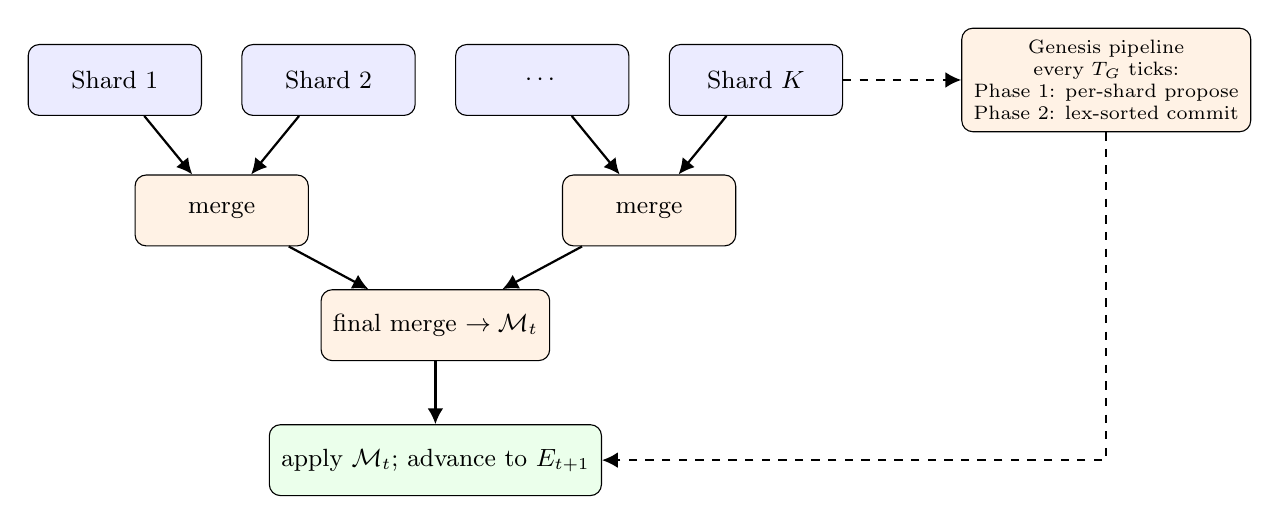
\begin{tikzpicture}[node distance=8mm and 5mm]
  \node[block, fill=blue!8] (s1) {Shard 1};
  \node[block, fill=blue!8, right=of s1] (s2) {Shard 2};
  \node[block, fill=blue!8, right=of s2] (s3) {$\cdots$};
  \node[block, fill=blue!8, right=of s3] (sk) {Shard $K$};

  \node[block, fill=orange!10, below=12mm of $(s1)!0.5!(s2)$] (m12) {merge};
  \node[block, fill=orange!10, below=12mm of $(s3)!0.5!(sk)$] (m34) {merge};
  \node[block, fill=orange!10, below=10mm of $(m12)!0.5!(m34)$] (mfinal) {final merge $\to \mathcal{M}_t$};

  \draw[arrow] (s1) -- (m12);
  \draw[arrow] (s2) -- (m12);
  \draw[arrow] (s3) -- (m34);
  \draw[arrow] (sk) -- (m34);
  \draw[arrow] (m12) -- (mfinal);
  \draw[arrow] (m34) -- (mfinal);

  \node[block, fill=green!8, below=8mm of mfinal] (apply) {apply $\mathcal{M}_t$; advance to $E_{t+1}$};
  \draw[arrow] (mfinal) -- (apply);

  \node[branchblock, right=15mm of sk, align=center, font=\scriptsize, minimum width=30mm] (genesis)
       {Genesis pipeline\\every $T_G$ ticks:\\Phase 1: per-shard propose\\Phase 2: lex-sorted commit};
  \draw[arrow, dashed] (sk.east) -- (genesis.west);
  \draw[arrow, dashed] (genesis.south) |- (apply.east);
\end{tikzpicture}
\caption{SLDM architecture. $K$ shards run drift, gate, compose, and emit independently each tick; emissions are reduced through a balanced binary tree of commutative-monoid merges. Every $T_G$ ticks the genesis pipeline runs in two phases: per-shard candidate proposal in parallel, then a sequential commit ordered by a lexicographic key over candidates.}
\label{fig:sldm}
\end{figure}

\subsection{Notation for this appendix}

\notationtable{Symbols introduced in this appendix.}{tab:notation-sldm}{
$K$                       & $\mathbb{N}$                 & number of shards (parallelism degree, fixed for the run) \\
$\Pi_k$                   & set of instances             & shard $k$'s slice of carrier instances \\
$\sigma_{\mathrm{shard}}$ & function                     & deterministic shard map: $\mathrm{Inst} \to \{1,\ldots,K\}$ \\
$\omega^{t}_{k,s}$        & $\Omega$                     & PRNG sub-stream for shard $k$, subsystem $s$, tick $t$ \\
$\mathrm{SplitMix}(\cdot)$ & function                    & stateless deterministic PRF used to derive sub-streams \\
$\mathcal{M}_t^{(k)}$     & multiset                     & per-shard emission multiset \\
$\mathrm{LSH}(\cdot)$     & hash family                  & locality-sensitive hash for slot signatures \\
$L_{\mathrm{bands}}, r_{\mathrm{rows}}$ & $\mathbb{N}$   & LSH parameters (bands, rows per band) \\
$\mathrm{lex}(\beta)$     & tuple                        & lexicographic admission key for bucket $\beta$ \\
$W$                       & cost                         & total work in PRAM-style analysis \\
$D$                       & cost                         & critical-path depth in PRAM-style analysis \\
}

\subsection{Shard partition}

We need to split the entities deterministically across workers. The partition function takes any instance id and returns a worker number. The key requirement is that the function be a deterministic function of the input state alone, so that two runs with identical inputs assign instances to the same shard regardless of how the run was launched. We use the lex-rank of the instance id modulo the shard count, which is the simplest rule that achieves this.

Define the shard map
\[
\sigma_{\mathrm{shard}}(B, i) \;=\; \mathrm{lex\_rank}(\mathrm{id}_B, \mathrm{id}_i) \bmod K,
\]
where $\mathrm{lex\_rank}$ is a deterministic ranking of instance ids. For carriers with spatial position, an effective alternative is to index by a Hilbert-curve embedding of the position; this preserves spatial locality across shards and reduces the cost of position-keyed primitive emissions. Either choice is admissible; the only requirement is that $\sigma_{\mathrm{shard}}$ is a deterministic function of the input state, independent of $K$ in its computation pattern (the modulus changes the resulting partition but the function is well-defined for any $K$).

Re-sharding (when instances are born or destroyed) recomputes $\sigma_{\mathrm{shard}}$ at instance birth/death events; instances do not migrate within a tick.

\subsection{PRNG stream split}

Each shard needs its own randomness, but the randomness must be reproducible regardless of how many shards exist. The naive approach --- advance a single global stream and hand chunks of it to each shard --- fails: the chunk shard $k$ receives depends on how many shards came before it, so the same shard sees different bytes at different parallelism degrees. The fix is a stateless hash function that takes the shard number as an explicit argument.

The model requires that randomness comes from named, seeded streams (\cref{sec:drift}). Under sharding we additionally derive per-(shard, subsystem, tick) sub-streams via a stateless pseudo-random function:
\[
\omega^{t}_{k,s} \;=\; \mathrm{SplitMix}\!\bigl(\mathrm{globalseed},\, k,\, \mathrm{hash}(s),\, t\bigr).
\]
SplitMix~\cite{steele2014splitmix} is a 64-bit splittable PRF; any cryptographic-strength PRF (e.g., SipHash, ChaCha20-derived) suffices. The split has three properties critical to determinism:
\begin{enumerate}[leftmargin=1.5em,nosep]
\item \emph{Independence across shards.} $\omega^t_{k,s}$ is uncorrelated with $\omega^t_{k',s}$ for $k \ne k'$.
\item \emph{$K$-invariance.} The sub-stream observed by shard $k$ at tick $t$ depends only on $(k, s, t)$, not on the total $K$. Two runs at $K = K_1$ and $K = K_2$ assign the same shard $k$ the same stream.
\item \emph{Seed-reproducibility.} The stream is recoverable from $(\mathrm{globalseed}, k, s, t)$ alone, so no PRNG state need be saved per shard.
\end{enumerate}

This is the design choice that lets a single shard's drift run identically whether the simulation is partitioned into 1, 100, or 10\,000 shards.

\subsection{Per-shard tick}

Each shard runs its own copy of the per-tick operator on its slice of instances. Because each instance's per-tick work depends only on its own state and the read-only environment, no two shards need to coordinate during the tick itself --- they only meet again at the merge step. The within-shard work is exactly the operator of \cref{sec:tick}; we just thread the shard's PRNG sub-stream through it.

The per-shard tick procedure is the operator of \cref{sec:tick} with the explicit stream argument. The within-shard ordering is preserved verbatim from \cref{def:drift}, \cref{def:effective}, and \cref{def:emission}.

\begin{verbatim}
procedure shard_tick(k, t, sigma_t^k, E_t):
    omega <- SplitMix(seed, k, "drift", t)

    // Drift: data-parallel across instances within shard
    for each (B, i) in Pi_k in lex order of (id_B, id_i):
        for each C in instance i's channels in id order:
            for each s in S_C cup {bot} in sorted order:
                (x_C^{(i,s,t+1)}, omega) <-
                    D_C(x_C^{(i,s,t)}, sigma_t(B,i), E_t, omega)

    // Gate, compose, emit: data-parallel across instances
    M_k <- empty multiset
    for each (B, i) in Pi_k in lex order of (id_B, id_i):
        for each C in instance i's channels in id order:
            for each s in S_C cup {bot} in sorted order:
                if Phi_C(sigma_{t+1}(B,i), E_t, s):
                    r <- clamp_{R_C}(x_C^{(i,s,t+1)})
                    for each h in H_C in id order:                  // sequential!
                        c_hat <- effective_value(partner(h),...)
                        r <- clamp_{R_C}(eta_{kappa_h}(r, c_hat, k_h, tau_h))
                        for each P in emits(h):
                            e <- (P, V_P, op_P, target(...),
                                  Pi_h(P, r, ...), cost_P)
                            M_k <- M_k uplus {e}
    return M_k
\end{verbatim}

The composition fold (the inner loop over $H_C$) is necessarily sequential per channel; the outer loops are not. On a multi-core CPU the outer loops parallelise via work-stealing over instance ranges; on GPU they parallelise as kernel launches with one warp per channel.

\subsection{Deterministic merge tree}

When the per-shard work is done, we have $K$ piles of emissions to combine into one. A balanced binary tree reduces them in $\log K$ depth, and because the merge operator is commutative-associative (\cref{lem:merge-comm}), the order in which the tree visits leaves is irrelevant for the final result. Fixing the tree's shape to be a balanced binary on the shard ids gives every node a deterministic combine order, which is what we need for cross-machine reproducibility.

Cross-shard emission reduction uses a balanced binary tree on shard ids, where the tree shape is fixed by $K$:

\begin{verbatim}
procedure merge_tree(M_1, ..., M_K):
    if K == 1:
        return finalise(M_1)
    let K' = floor(K/2)
    L = merge_tree(M_1, ..., M_{K'})              // left subtree, parallel
    R = merge_tree(M_{K'+1}, ..., M_K)            // right subtree, parallel
    return monoid_combine(L, R)                   // commutative-monoid merge
\end{verbatim}

The combine operator is the merge monoid of \cref{lem:merge-comm}: associative and commutative on parameter values for each $(P, V_P, \mathrm{target})$ key. By \cref{lem:merge-comm}, the result is independent of the tree shape \emph{provided the monoid is exactly associative}. This holds for integer arithmetic, fixed-point arithmetic, and the kernel-supplied operators $\mathrm{sum}, \mathrm{max}, \mathrm{mean}, \mathrm{union}$. For floating-point parameters, exact associativity does not hold; we therefore require fixed-point arithmetic in the merge step for cross-$K$ replay invariance. This is consistent with the determinism preconditions of \cref{sec:properties}.

The tree is implemented by \texttt{MPI\_Reduce} on a cluster, by \texttt{rayon::reduce} (or equivalent) on multi-core CPU, and by a parallel scan primitive on GPU.

\subsection{Distributed genesis}

Genesis is the harder case for parallelisation, because bucket clustering naturally wants global information --- ``find me all agents whose latent slots agree.'' The naive approach is all-pairs similarity, which is $O(N^2)$ and never scales. We replace it with locality-sensitive hashing: agents with close signatures land in the same hash bucket with high probability, and we only do further comparisons within a bucket. This turns the global problem into a local one: each shard hashes its own agents, then we union the hash-bucket contents across shards. Admission of new channels into the registry is then sequential by design, but ordered by a deterministic key over candidates so that the final outcome is independent of which shard proposed which bucket.

The genesis transition every $T_G$ ticks runs in two phases.

\paragraph{Phase 1: locality-sensitive bucketing.}
The original pipeline of \cref{sec:gtrans} step~1 partitions agents by signature similarity, naively requiring $O(N^2)$ comparisons. We replace this with locality-sensitive hashing (LSH)~\cite{indyk1998}: each agent's top latent slot signature $\mathbf{u}_a$ is hashed into $L_{\mathrm{bands}}$ bands of $r_{\mathrm{rows}}$ rows. Agents collide in a band iff their $\mathbf{u}$'s project to the same hyperplane partition for that band; collision in $\geq 1$ band indicates likely closeness in $\mathbf{u}$. The hash family seed is part of the PRNG namespace, so the bucketing is deterministic across runs.

\begin{verbatim}
procedure lsh_bucket_local(k, t, agents_in_shard_k):
    H_seed = SplitMix(seed, "lsh", t)
    local_buckets[k] = {}
    for each a in agents_in_shard_k:
        for band b = 1 to L_bands:
            h = LSH_band(u_a, b, H_seed)
            local_buckets[k][(b, h)].insert(a)
    return local_buckets[k]
\end{verbatim}

The work is $O(N \cdot L_{\mathrm{bands}})$ total (so $O(N L_{\mathrm{bands}}/K)$ per shard), and depth is $O(L_{\mathrm{bands}})$.

\paragraph{Phase 2: cross-shard gather and lex-sorted commit.}
Local buckets are merged across shards by hashed bucket id; eligibility ($|\beta| \geq n_{\min}$) is checked on the merged bucket; per-bucket proposal then runs in parallel across eligible buckets. The non-trivial step is admission, which must be deterministic regardless of $K$:

\begin{verbatim}
procedure genesis_distributed(t):
    // (1) per-shard latent-pressure update has run every tick already.

    // (2) LSH bucketing -- parallel
    local_b = parallel_for k in 1..K: lsh_bucket_local(k, t, ...)

    // (3) Cross-shard merge of LSH buckets -- deterministic gather
    global_b = {}
    for (band, h) in lex order over all observed (band, h) keys:
        agents_bh = union over k of local_b[k][(band, h)]
        if |agents_bh| >= n_min:
            global_b[(band, h)] = agents_bh

    // (4) Per-bucket candidate proposal -- parallel
    candidates = parallel_for beta in global_b:
        omega_beta = SplitMix(seed, "genesis", t, hash(beta))
        Cmp = propose_composition(beta, omega_beta)
        Lat = propose_latent_extraction(beta)
        Mut = propose_mutation(beta, omega_beta)
        winner = argmax over m in {Cmp, Lat, Mut} of fitness(m, beta)
        return (lex(beta), beta, winner)

    // (5) Deterministic admission -- sequential, sorted by lex key
    sort candidates by lex key ascending
    for (key, beta, winner) in sorted order:
        if fitness(winner) >= q_min and qd_admits(winner, archive):
            new_id = "genesis:" + omega_beta + ":" + t + ":" + kappa
                     + ":" + H(u_beta, sort(par), mechanism)
            C_t  := C_t  union {winner}
            L_t  := L_t  concat g_beta
            archive := admit(winner, archive)

    // (6) Replicate registry and lineage to every shard
    broadcast(C_t, L_t)
\end{verbatim}

The lex key $\mathrm{lex}(\beta) = (t, \omega_\beta, \mathrm{hash}(\mathbf{u}_\beta))$ totalises buckets so that admission order is independent of which shard proposed a bucket first. The sequential admission loop is the only Amdahl bottleneck in the pipeline; with $T_G \sim 10^3$ and $|B| \sim 10^3$ buckets per pass, its amortised per-tick cost is below 1\% of total work.

\subsection{Determinism}

The whole point of the SLDM construction is the next theorem: it doesn't matter how many shards you use --- the simulation produces byte-identical state. This is what makes the replay guarantee from \cref{sec:properties} survive parallelisation. A user who debugged a problem at $K = 1$ on a laptop can rerun at $K = 1024$ on a cluster and see exactly the same state evolve.

\begin{theorem}[Replay invariance under parallelism]\label{thm:sldm-det}
Let $\Sigma^{(K)}_{t+1}$ denote the post-tick world state produced by the SLDM algorithm with $K$ shards from inputs $(\Sigma_t, E_t, \mathrm{globalseed})$. Then for any $K_1, K_2 \in \mathbb{N}_{\ge 1}$,
\[
\Sigma^{(K_1)}_{t+1} \;=\; \Sigma^{(K_2)}_{t+1}.
\]
\end{theorem}

\begin{proof}
By induction on $t$, with the base case $\Sigma_0$ given. For the inductive step, four properties must hold:
\begin{enumerate}[leftmargin=1.5em,nosep]
\item Within-shard ordering reproduces the operator of \cref{sec:tick} verbatim, by the construction of \texttt{shard\_tick}.
\item PRNG sub-streams depend only on $(k, s, t, \mathrm{globalseed})$, by the SplitMix derivation. They do not depend on $K$.
\item Cross-shard reduction uses a commutative monoid (\cref{lem:merge-comm}); under fixed-point arithmetic the monoid is exactly associative, so any tree shape yields the same result. In particular the balanced binary tree of \texttt{merge\_tree} yields the same byte string for any $K$.
\item Genesis admission is sequential and ordered by the deterministic lex key, so its result is independent of which shard proposed which bucket and of the total shard count.
\end{enumerate}
The composition of these four operations is therefore $K$-invariant, completing the induction.
\end{proof}

A subtler corollary: because \texttt{merge\_tree} relies on \emph{exact} associativity of the merge monoid, IEEE-754 floating-point parameter values break the theorem when $K$ varies (they do not break it when $K$ is held fixed). Bit-identical replay across arbitrary $K$ therefore requires fixed-point arithmetic for any parameter that flows through merge, which is consistent with the determinism preconditions of \cref{sec:properties}.

\subsection{Complexity and scaling}

In PRAM-style notation with total work $W$ and critical-path depth $D$:

\begin{table}[ht]
\centering
\caption{Per-tick work and depth for the SLDM algorithm. $N$: number of carrier instances; $|H|$: bounded hooks per channel; $K$: shard count.}
\label{tab:sldm-cost}
\small
\begin{tabularx}{\linewidth}{l l Y}
\toprule
Stage & $W$ & $D$ \\
\midrule
Drift                          & $O(N|H|)$                    & $O(|H|)$ \\
Gate evaluation                & $O(N)$                       & $O(1)$ \\
Composition fold               & $O(N|H|)$                    & $O(|H|)$ \\
Emission                       & $O(N|H|)$                    & $O(1)$ \\
Merge tree                     & $O(N)$                       & $O(\log K)$ \\
\midrule
\emph{Per-tick total}          & $O(N|H|)$                    & $O(|H| + \log K)$ \\
\bottomrule
\end{tabularx}
\end{table}

\begin{table}[ht]
\centering
\caption{Genesis-pass work and depth, amortised per tick by dividing by $T_G$. $B$: buckets per pass; $|\Omega|$: composition operators per kind; $K_a$: latent-slot bound per agent; $L_{\mathrm{bands}}$: LSH bands.}
\label{tab:sldm-genesis-cost}
\small
\begin{tabularx}{\linewidth}{l l Y}
\toprule
Stage & $W$ (per pass) & $D$ (per pass) \\
\midrule
Latent update (per tick)       & $O(N K_a)$                   & $O(K_a)$ \\
LSH bucketing                  & $O(N L_{\mathrm{bands}})$    & $O(L_{\mathrm{bands}})$ \\
Cross-shard merge of buckets   & $O(N)$                       & $O(\log K)$ \\
Per-bucket proposal            & $O(B \cdot |\Omega| \cdot |\mathcal{C}|)$ & $O(|\Omega| \cdot |\mathcal{C}|)$ \\
Sequential QD admission        & $O(B \log B)$                & $O(B)$ \\
\bottomrule
\end{tabularx}
\end{table}

The sequential admission is the only Amdahl bottleneck. With representative parameters ($N = 10^7$, $B = 10^3$, $T_G = 10^3$), its amortised per-tick depth is $O(1)$ and well under 1\% of per-tick work.

The expected speedup with $K$ workers is
\[
S(K) \;=\; \frac{W}{W/K + D + W_{\mathrm{seq}}/T_G}
\;\approx\; \frac{K}{1 + (K \log K + K B)/(N |H|)}
\]
which is approximately linear in $K$ as long as $K \log K \ll N|H|$. For $N = 10^9, |H| = 8, K = 10^4$, this gives near-linear speedup; for $N = 10^6, |H| = 8, K = 10^4$, the merge tree begins to dominate.

\subsection{Hardware-tier mapping}

\begin{table}[ht]
\centering
\caption{The same SLDM algorithm runs at three hardware tiers; only the synchronisation primitives differ.}
\label{tab:sldm-tiers}
\small
\begin{tabularx}{\linewidth}{l L{0.32\linewidth} Y}
\toprule
Tier & Shard model & Sync primitives \\
\midrule
Multi-core CPU, 1 node    & one shard per worker thread & work-stealing pool; \texttt{rayon::reduce} for merge tree; shared-memory broadcast \\
Distributed cluster       & one shard per MPI rank      & \texttt{MPI\_Reduce} for merge tree; \texttt{MPI\_Allgather} or \texttt{MPI\_Bcast} for genesis broadcast \\
Hybrid CPU+GPU, 1 node    & one shard per CUDA stream / one rank for CPU-side genesis & per-shard tick on GPU; merge tree, QD admission, lineage on CPU; double-buffered ticks for CPU--GPU pipeline \\
\bottomrule
\end{tabularx}
\end{table}

The same source code can target all three tiers via a thin synchronisation abstraction (one trait or interface with three implementations).

\subsection{GPU acceleration notes}

\begin{table}[ht]
\centering
\caption{Per-stage GPU acceleration suitability.}
\label{tab:sldm-gpu}
\small
\begin{tabularx}{\linewidth}{l l Y}
\toprule
Stage & GPU fit & Notes \\
\midrule
Drift fold                     & Excellent & data-parallel, regular memory; one CUDA thread per (instance, channel, site) \\
Gate evaluation                & Excellent & branchless when predicates expressed as masks \\
Composition fold               & Good      & sequential within a channel; one warp per channel keeps the SIMT unit fed \\
Emission                       & Good      & stream-compaction kernel (CUB \texttt{DeviceSelect}) \\
Merge tree (intra-shard)       & Excellent & parallel reduce primitive (CUB \texttt{DeviceReduce}) \\
Merge tree (inter-shard)       & Mixed     & cross-device communication via NVLink/RDMA preferred; CPU-staged otherwise \\
LSH bucketing                  & Excellent & hash kernel + radix sort \\
Latent extraction              & Excellent & power iteration in cuBLAS \\
Mutation perturbation          & Good      & one thread per candidate \\
QD admission                   & Avoid     & sequential, low arithmetic intensity \\
Lineage append, broadcast      & Avoid     & I/O-bound \\
\bottomrule
\end{tabularx}
\end{table}

The recommended split is per-shard tick stages on GPU, with cross-shard reduction, QD admission, and lineage append on CPU. CPU and GPU pipeline across consecutive ticks: while the GPU computes shard ticks for tick $t+1$, the CPU finalises merge and (when scheduled) genesis admission for tick $t$.

\subsection{Tradeoffs}

\begin{table}[ht]
\centering
\caption{SLDM design choices and rationale.}
\label{tab:sldm-rationale}
\small
\begin{tabularx}{\linewidth}{L{0.28\linewidth} L{0.28\linewidth} Y}
\toprule
Choice & Alternatives & Rationale \\
\midrule
Static shard partition (lex-rank mod $K$ or Hilbert curve)
& Dynamic load balancing per tick; work stealing across all instances
& Static partition is deterministic for any $K$; dynamic balancing introduces nondeterminism unless the balancing decisions are themselves derived from inputs. The static partition is rebalanced only at instance birth/death, deterministically. \\
Per-(shard, subsystem, tick) PRNG via SplitMix
& Per-shard streams advanced from a single global stream
& SplitMix gives $K$-invariance: shard $k$'s stream depends on $k$ explicitly. A globally-advanced stream would correlate sub-streams in a way that depends on shard scheduling, breaking replay invariance. \\
Balanced binary merge tree
& Linear left-fold; ring reduce; recursive doubling
& All four are $O(\log K)$ depth and yield identical results under exact associativity. The balanced binary tree minimises the depth's dependence on $K$, fits MPI's collective implementations, and is what every parallel-reduce library defaults to. \\
LSH bucketing
& All-pairs similarity; $k$-means; spectral clustering
& All-pairs is $O(N^2)$ and cannot scale; $k$-means and spectral methods are not deterministic without seeded initialisation, and produce buckets that depend on iteration count. LSH is $O(N)$ and deterministic given the hash family seed. \\
Lex-sorted sequential QD admission
& Per-shard archives; locks on a global archive
& Per-shard archives fragment diversity (different shards admit overlapping candidates). Locks introduce nondeterminism through scheduling. Sequential admission ordered by a deterministic key gives a single admission decision invariant to $K$. \\
Replicated $L_t$ and $\mathcal{C}_t$ across shards
& Centralised lineage server; per-shard lineage shards
& Replication is cheap ($L_t$ is small and grows slowly) and lets each shard make admission decisions locally during the next tick without round-tripping. A centralised server adds RPCs to the per-tick path. \\
Disallow within-tick instance migration across shards
& Periodic migration; per-tick re-sharding
& Migration introduces ordering dependencies between shards within a tick, breaking the embarrassingly-parallel property. Re-sharding only at birth/death keeps the within-tick partition stable. \\
\bottomrule
\end{tabularx}
\end{table}

\subsection{Open engineering questions}

\begin{enumerate}[leftmargin=1.5em,nosep]
\item \emph{Re-sharding policy.} How often to recompute $\sigma_{\mathrm{shard}}$ when the population grows? Renumbering all instances on every birth is expensive; deferring renumbering risks load imbalance. A reasonable policy is to renumber whenever shard load deviates by more than a threshold from the mean, deterministically scheduled.
\item \emph{Merge-tree topology.} Binary trees minimise depth; $k$-ary trees minimise communication count. Optimal choice depends on the network's latency-vs-bandwidth profile and on the merge-monoid's combine cost.
\item \emph{LSH parameter tuning.} The pair $(L_{\mathrm{bands}}, r_{\mathrm{rows}})$ controls the recall--precision tradeoff in bucketing; tuning is empirical and depends on the typical structure of $\mathbf{u}$ across populations. A self-tuning scheme could adjust these parameters based on the per-tick admission rate.
\item \emph{Snapshot frequency.} Crash recovery via replay-from-seed costs $O(t)$; periodic snapshots cost $O(|\Sigma_t|)$ in storage but bound recovery time. The tradeoff depends on tick rate and storage bandwidth.
\item \emph{Cross-shard primitive emissions.} Field-typed world variables (\cref{sec:emit}) are spatial and may be written by primitives whose target lies in another shard. The current scheme either replicates field state across shards (memory cost) or routes emissions through a shard-local proxy that forwards at merge time (latency cost).
\item \emph{Determinism under hardware float reordering.} GPUs reorder floating-point operations at the warp level. Using fixed-point throughout is the safe choice; if floats are unavoidable for performance reasons, the cross-$K$ replay guarantee weakens to ``cross-run replay at fixed $K$''.
\end{enumerate}

% =========================================================================
\begin{thebibliography}{99}

\bibitem{wagner2011}
A.~Wagner, \emph{The Origins of Evolutionary Innovations}.
Oxford, UK: Oxford University Press, 2011.

\bibitem{stanley2007}
K.~O.~Stanley,
``Compositional pattern producing networks: a novel abstraction of development,''
\emph{Genetic Programming and Evolvable Machines}, vol.~8, no.~2, pp.~131--162, 2007.

\bibitem{friston2010}
K.~Friston,
``The free-energy principle: a unified brain theory?''
\emph{Nature Reviews Neuroscience}, vol.~11, no.~2, pp.~127--138, 2010.

\bibitem{griffiths2011}
T.~L.~Griffiths and Z.~Ghahramani,
``The Indian buffet process: an introduction and review,''
\emph{Journal of Machine Learning Research}, vol.~12, pp.~1185--1224, 2011.

\bibitem{arthur2009}
W.~B.~Arthur, \emph{The Nature of Technology: What It Is and How It Evolves}.
New York, NY: Free Press, 2009.

\bibitem{lake2015}
B.~M.~Lake, R.~Salakhutdinov, and J.~B.~Tenenbaum,
``Human-level concept learning through probabilistic program induction,''
\emph{Science}, vol.~350, no.~6266, pp.~1332--1338, 2015.

\bibitem{lehman2011}
J.~Lehman and K.~O.~Stanley,
``Evolving a diverse set of virtual creatures through novelty search and local competition,''
in \emph{Proc.\ Genetic and Evolutionary Computation Conf.\ (GECCO)}, 2011, pp.~211--218.

\bibitem{mouret2015}
J.-B.~Mouret and J.~Clune,
``Illuminating search spaces by mapping elites,''
arXiv:1504.04909, 2015.

\bibitem{lim2025}
B.~Lim et al.,
``Dominated novelty search: rethinking local competition in quality--diversity,''
arXiv:2502.00593, 2025.

\bibitem{lijoi2023}
A.~Lijoi, R.~H.~Mena et al.,
``Bayesian analysis of generalized hierarchical Indian buffet processes for within and across group sharing of latent features,''
arXiv:2304.05244, 2023.

\bibitem{bedau1998}
M.~A.~Bedau, E.~Snyder, and N.~H.~Packard,
``A classification of long-term evolutionary dynamics,''
in \emph{Proc.\ Artificial Life VI}, 1998, pp.~228--237.

\bibitem{soros2014}
L.~B.~Soros and K.~O.~Stanley,
``Identifying necessary conditions for open-ended evolution through the artificial life world of Chromaria,''
\emph{Artificial Life}, vol.~14, pp.~793--800, 2014.

\bibitem{drescher1991}
G.~L.~Drescher, \emph{Made-up Minds: A Constructivist Approach to Artificial Intelligence}.
Cambridge, MA: MIT Press, 1991.

\bibitem{steele2014splitmix}
G.~L.~Steele, D.~Lea, and C.~H.~Flood,
``Fast splittable pseudorandom number generators,''
in \emph{Proc.\ ACM SIGPLAN Conf.\ on Object-Oriented Programming, Systems, Languages, and Applications (OOPSLA)}, 2014, pp.~453--472.

\bibitem{indyk1998}
P.~Indyk and R.~Motwani,
``Approximate nearest neighbors: towards removing the curse of dimensionality,''
in \emph{Proc.\ 30th ACM Symposium on Theory of Computing (STOC)}, 1998, pp.~604--613.

\end{thebibliography}

\end{document}
